% autosam.tex
% Annotated sample file for the preparation of LaTeX files
% for the final versions of papers submitted to or accepted for 
% publication in AUTOMATICA.

% See also the Information for Authors.

% Make sure that the zip file that you send contains all the 
% files, including the files for the figures and the bib file.

% Output produced with the elsart style file does not imitate the
% AUTOMATICA style. The style file is generic for all Elsevier
% journals and the output is laid out for easy copy editing. The
% final document is produced from the source file in the
% AUTOMATICA style at Elsevier.

% You may use the style file autart.cls to obtain a two-column 
% document (see below) that more or less imitates the printed 
% Automatica style. This may helpful to improve the formatting 
% of the equations, tables and figures, and also serves to check 
% whether the paper satisfies the length requirements.

% Please note: Authors must not create their own macros.

% For further information regarding the preparation of LaTeX files 
% for Elsevier, please refer to the "Full Instructions to Authors" 
% from Elsevier's anonymous ftp server on ftp.elsevier.nl in the
% directory pub/styles, or from the internet (CTAN sites) on
% ftp.shsu.edu, ftp.dante.de and ftp.tex.ac.uk in the directory
% tex-archive/macros/latex/contrib/supported/elsevier.
% \documentclass{elsart}               % The use of LaTeX2e is preferred.
\documentclass[onecolumn]{autart}    
% Enable this line and disable the 
% preceding line to obtain a two-column 
% document whose style resembles the
% printed Automatica style.


\usepackage{graphicx}
\usepackage{dsfont}
\usepackage{color}
\usepackage{amsfonts,amsmath}
\usepackage{caption}
\usepackage{subcaption}
\usepackage{hyperref}
\usepackage{float}
\captionsetup[subfigure]{labelformat = parens, labelsep = space, font = small}
\usepackage{tikz,pgf}

\usepackage{pgfplots} 

\newtheorem{proof}{Proof}
%\newtheorem{theorem}{Theorem}[section]
%\newtheorem{lemma}[theorem]{Lemma}
%\newtheorem{proposit}[theorem]{Proposition}
%\newtheorem{corollary}[theorem]{Corollary}
%\newtheorem{remark}[theorem]{Remark}
%\newtheorem{example}[theorem]{Example}
%\newtheorem{assumption}[theorem]{Assumption}

\newcommand{\lan}{\langle}
\newcommand{\ran}{\rangle}
\newcommand{\R}{\mathbb{R}}
\newcommand{\E}{\mathbb{E}}
\newcommand{\Law}{\mathcal{L}}
\newcommand{\Z}{\mathbb{Z}}
\newcommand{\1}{\mathds{1}}
%\usepackage[dvips]{epsfig}    
% or this line, depending on which
% you prefer.
\allowdisplaybreaks
\begin{document}

\begin{frontmatter}
%\runtitle{Modified Euler schemes for MVSDE}  
% Running title for regular 
% papers but only if the title  
% is over 5 words. Running title 
% is not shown in output.

\title{On modified Euler methods for McKean-Vlasov stochastic differential equations with super-linear coefficients\thanksref{footnoteinfo}} 
% Title, preferably not more 10 words

\thanks[footnoteinfo]{
Corresponding author: Qingshuo Song. All authors contributed equally.}

\author[UM]{Jiamin Jian}\ead{jiaminj@umich.edu},    
\author[WPI]{Qingshuo Song}\ead{qsong@wpi.edu},    
\author[CS]{Xiaojie Wang}\ead{x.j.wang7@csu.edu.cn},
\author[WPI]{Zhongqiang Zhang}\ead{zzhang7@wpi.edu}, 
\author[CS]{Yuying Zhao}\ead{zhaoyuying78@gmail.com} 

\address[UM]{Department of Mathematics, University of Michigan, Ann Arbor, MI 48109, USA}  

\address[WPI]{Department of Mathematical Sciences, Worcester Polytechnic Institute, Worcester, MA 01609, USA}  

\address[CS]{School of Mathematics and Statistics, HNP-LAMA, Central South University, Changsha, Hunan, P. R. China} 


% Please supply full addresses here.
                                         
%\address[CS]{School of Mathematics and Statistics, HNP-LAMA, Central South University, Changsha, Hunan, P. R. China}             
          
\begin{keyword}                           
% Five to ten keywords,  
McKean–Vlasov SDEs, mean-field models, interacting particle system, modified Euler methods, propagation of chaos.
% chosen from the IFAC 
\end{keyword}                             
% keyword list or with the 
% help of the Automatica 
% keyword wizard
\begin{abstract}                          
% Abstract of not more than 200 words.
We introduce a new class of numerical methods for solving McKean-Vlasov stochastic differential equations, which are relevant in the context of distribution-dependent or mean-field models, under super-linear growth conditions for both the drift and diffusion coefficients. Under certain non-globally Lipschitz conditions, the proposed numerical approaches have half-order convergence in the strong sense to the corresponding system of interacting particles associated with  McKean-Vlasov SDEs. By leveraging a result on the propagation of chaos, we establish the full convergence rate of the modified Euler approximations to the solution of the McKean-Vlasov SDEs. Numerical experiments are included to validate the theoretical results.
\end{abstract}

\end{frontmatter}

\section{Introduction}

McKean-Vlasov stochastic differential equations (MV-SDEs), also known as distribution-dependent or mean-field SDEs, extend traditional SDEs by incorporating the collective behavior of multiple interacting particles. 
Initially proposed by McKean \cite{mckean1966class}, \cite{mckean1967propagation}, this class of equations gained increasing attention following Dawson’s foundational work \cite{dawson1983critical} and the development of the Lion's derivative with respect to the measure variables \cite{lions2007cours}. 
Solving MV-SDEs is crucial in control theory as they model large-scale systems where individual components interact with the collective behavior of the group. They describe both the optimal path for mean-field controls \cite{bensoussan2013mean}, \cite{sznitman1991topics} and the equilibrium trajectory for mean-field games (see \cite{CD18I}, \cite{CD18II}, \cite{Mishura20}, \cite{wu2022stabilization} and references therein). This type of SDEs are essential for simplifying control problems in distributed systems, such as robots, power grids, or financial markets, by focusing on the statistical distribution of agents rather than individual interactions. They also account for uncertainty in noisy environments, enabling robust control strategies. Applications include multi-agent systems (see \cite{Benachour98}, \cite{Bossy97}) and other highly relevant fields like filtering (as highlighted in \cite{Crisan10}). By reducing system complexity and providing feedback control for distributed systems, MV-SDEs make large-scale optimization problems more tractable.


McKean–Vlasov SDEs are also widely used to model random phenomena across various scientific domains, including physics, biology, engineering, and neural activities, such as \cite{Baladron12}, \cite{Bolley11}, \cite{Bossy15}, \cite{CD18I}, \cite{CD18II}, \cite{Dreyer11}, \cite{Guhlke18}, \cite{mckean1966class} and references therein. As a result, there has been a notable surge in interest in related research.



Let $(\Omega, \mathcal{F}, \{ \mathcal{F}_t\}_{ t \geq 0 }, \mathbb{P})$ be a filtered probability space satisfying the usual conditions, where $\mathcal F_t$ is the augmented filtration of a standard $m$-dimensional Brownian motion $W = \{W(t)\}_{t \geq 0}$.
For a fixed terminal time $T > 0$, we consider the following McKean–Vlasov SDEs
\begin{equation}
\label{eq:MV_SDE}
X_t = X_0 + \int_0^t b \left(s, X_s,  \Law (X_s) \right) ds + \int_0^t \sigma \left(s, X_s,  \Law (X_s) \right) d W(s), \quad
t \in [0, T],
\ a.s.,
\end{equation}
where $\{\Law (X_t)\}_{t \geq 0}$ is the flow of deterministic marginal distributions of $X = \{X_t\}_{t \geq 0}$, $b:[0, T] \times \R^d \times \mathcal P_2(\R^d) \to \R^d$ denotes the drift function and $\sigma:[0, T] \times \R^d \times \mathcal P_2(\R^d) \to \R^{d \times m}$ is the diffusion function, expressed as $\sigma = (\sigma_1, \sigma_2, \dots, \sigma_m)$.
In this notation, $\sigma_j: [0, T] \times \R^d \times \mathcal P_2(\R^d) \to \R^{d}$ is the $j$-th column of $\sigma$.
\iffalse
Then, the McKean–Vlasov SDEs \eqref{eq:MV_SDE} can also be written by
\begin{equation*}
X_t = X_0 + \int_0^t b \left(s, X_s,  \Law (X_s) \right) ds + \sum_{j = 1}^{m} \int_0^t \sigma_{j} (s, X_s,  \Law (X_s)) d W_j (s),
\, \,
t \in [0, T],
\quad a.s.
\end{equation*}
\fi
Throughout this paper, the initial data
$X_0$ is a $\mathcal F_0$-measurable random variable in $\R^d$ independent of $W$.

\iffalse
The considered MV-SDEs \eqref{eq:MV_SDE} are commonly employed to mathematically model random phenomena originating from various scientific fields, including physics, biology, engineering, and neural activities, such as \cite{Baladron12}, \cite{Bolley11}, \cite{Bossy15}, \cite{CD18I}, \cite{CD18II}, \cite{Dreyer11}, \cite{Guhlke18}, \cite{Mckean66} 
and references therein. 
Moreover, 
MV-SDEs, characterized by their greater complexity compared to It\^o's stochastic differential equations, emerge in various theoretical contexts, including multi-agent systems (see \cite{Benachour98}, \cite{Bossy97}) and other highly relevant domains like filtering (as highlighted in \cite{Crisan10}). 
Specifically, it is noteworthy that the optimal path for mean-field controls and the equilibrium trajectory for mean-field games can often be described as MV-SDEs, see \cite{CD18I}, \cite{CD18II}, \cite{Mishura20} and references therein. As a result, there has been a notable surge in interest in related research.
\fi


In general, such equations rarely have explicit solutions available and one usually falls back on their numerical solutions. If the measure flow $\{\Law (X_t)\}_{t \geq 0}$ is known, then the coefficients $b$ and $\sigma$ are functions of time and space variables, and hence the MV-SDEs reduce to classical SDEs.
It is widely acknowledged that in scenarios where the coefficients of SDEs lack globally Lipschitz continuity and exhibit super-linear growth, the commonly used Euler-Maruyama numerical solution fails to attain finite moments, leading to divergence in both strong and weak senses. This issue has been well-documented in the literature, as evidenced by, e.g., \cite{Higham07}, \cite{Hutzen11}, \cite{Matting02},
\cite{KS17} and \cite{Mils05}. A similar divergence phenomenon, referred to as particle corruption, was observed in the context of MV-SDEs (see Section 4.1 in \cite{Reis22} for more details). 
%The authors demonstrate that a single particle can destabilize the entire system, with the likelihood of such an event increasing as the number of particles grows. For further details, see Section 4.1 in \cite{Reis22}.
Therefore, special care must be taken to construct and analyze convergent numerical approximations in a non-globally Lipschitz setting and recent years have witnessed a proper growth of the literature on this interesting topic \cite{Bao21},
\cite{liu2023tamed}, \cite{Reis22}, 
\cite{chen2022flexible}, \cite{gao2024convergence}, \cite{KN21}, \cite{Kumar22}, \cite{LMSWY23}, \cite{Liu23}, \cite{Neelima20}, \cite{chen2024euler}, \cite{chen2023wellposedness} and \cite{reisinger2022adaptive}.

\iffalse
Particularly, tamed Milstein-type numerical method \cite{Bao21}, \cite{KN21} appeared concurrently for the interacting particle system associated with the MV-SDEs while the drift coefficient is still allowed to grow super-linearly in the state variable, the diffusion coefficient satisfies global Lipschitz continuity condition in the state variable and both the coefficients are assumed to be global Lipschitz continuous in the measure component.
\fi

Under local Lipschitz and linear growth conditions, the Euler numerical method for approximating MV-SDEs was analyzed in \cite{LMSWY23}. When the drift coefficients exhibit possible super-linear growth while the diffusion coefficients satisfy the linear growth condition, the moment boundedness and convergence rates of various numerical methods have been investigated in \cite{Bao21}, \cite{Reis22}, \cite{reisinger2022adaptive},\cite{fang2020adaptive}, \cite{KN21}, and 
\cite{liu2023tamed}. 
This analysis was further extended in \cite{Kumar22} to MV-SDEs with common noise and in \cite{Neelima20} to those with L\'evy processes, allowing the diffusion coefficients to also exhibit super-linear growth.
In addition, numerical methods have been proposed for solving a class of MV-SDEs with drift or diffusion components of convolution type. Specifically, \cite{chen2022flexible} and \cite{chen2024euler} addressed cases where both drifts and diffusions exhibit super-linear growth, while \cite{chen2023wellposedness} focused on drifts with super-linear growth and diffusion coefficients satisfying linear growth conditions. Finally, some works addressed numerical methods for McKean–Vlasov SDEs with H\"older continuous diffusion coefficient (see, e.g., \cite{Liu23}).
In terms of numerical methods, various approaches have been proposed in the literature:

%Under local Lipschitz and linear growth conditions, \cite{LMSWY23} investigates the Euler numerical method for approximating MV-SDEs.
%When the drift coefficients possibly grow super-linearly and the diffusion coefficients obey the linear growth condition, 
%the tamed Euler numerical method is applied by \cite{gao2024convergence} to approximate a type of highly nonlinear neutral multiple-delay MV-SDEs.  
%MV-SDEs
%moment boundedness and convergence rates of several various numerical methods have been studied in \cite{Bao21}, \cite{Reis22}, \cite{reisinger2022adaptive},\cite{fang2020adaptive}, \cite{KN21}, and 
%\cite{liu2023tamed}. 
%\textcolor{red}{The above analysis is extended to MV-SDEs with common noise in \cite{Kumar22} and with L\'evy process in \cite{Neelima20}, allowing the diffusion coefficient to also exhibit super-linear growth. 
%In addition to the aforementioned explicit methods, some implicit numerical methods such as split-step Euler-type methods have been proposed to solve a class of MV-SDEs with drift or diffusion components of convolution type (see \cite{chen2022flexible}, \cite{chen2024euler}, and \cite{chen2023wellposedness}).} 
\begin{itemize}
\item 
\textit{Explicit tamed Euler methods}, were introduced and studied in  \cite{Reis22}, \cite{liu2023tamed}, \cite{Liu23}, \cite{Neelima20}, \cite{Bao21}, \cite{KN21}, and \cite{Kumar22}, which rely on certain taming modifications of coefficients of MV-SDEs in a form such as $\frac{b(t, x, \mu)}{1+h^{\beta}|b(t, x, \mu)|} \, (0 < \beta \leq 1)$; 
%In \cite{Kumar22}, a tamed scheme is proposed for MV-SDE featuring common noise in the particle system 
%and where the diffusion is also allowed to grow superlinearly.

%\item 
%Milstein-type \textcolor{red}{numerical solution}, \cite{Bao21}, \cite{KN21},  appeared concurrently for the interacting particle system associated with the McKean–Vlasov SDEs  while the drift coefficient is still allowed to grow super-linearly in the state variable, the diffusion coefficient satisfies global Lipschitz continuity condition in the state variable and both the coefficients are assumed to be global Lipschitz continuous in the measure component;

\item 
\textit{Adaptive numerical methods} may serve as a viable alternative to tamed numerical solutions, particularly in numerically solving super-linear drift and diffusion coefficients, as demonstrated in \cite{reisinger2022adaptive};
%, and \cite{kelly2023strong};}

\item 
\textit{Truncated method} was proposed in \cite{guo2024convergence} for the interacting particle system under a Khasminskii-type condition on the coefficients;

\item 
\textit{Projection-based particle method} was proposed in \cite{belomestny2018projected} to reduce the computational cost of solving MV-SDEs;

\item
\textit{Implicit numerical methods}, such as the backward Euler method \cite{Reis22} and 
\textit{split-step method} (see \cite{chen2022flexible}, \cite{chen2024euler}, \cite{chen2023wellposedness})
%which combine implicit and explicit techniques, 
were utilized to approximate MV-SDEs with superlinear coefficients.
\end{itemize}

%
%Notably tamed numerical methods have been studied in \cite{Kumar22} and \cite{Neelima20} under a weaker assumption that the diffusion coefficients are also of super-linear growth. 
It is worthwhile to note that, when numerically approximating stable (dissipativity) systems, stability (or dissipativity) preserving methods are particularly vital. Usually, implicit methods have excellent stability properties and can preserve the dissipativity (long time stability) of the system, but at a price of expensive costs. 
A cheap option is to rely on explicit methods. 
However, as pointed out by \cite{chen2022flexible}, taming might destroy the strict dissipativity of the drift coefficients
and the usual tamed methods would be confronted with long time stability issues.
Our numerical experiments indicate different taming strategies would give different stability performances. 
%New taming strategies are thus needed to overcome this issue, 
Therefore, one should be careful with the choice of taming strategies for long-time simulations,
which, albeit interesting and important, turns out to be non-trivial.
Recently, several authors have made some attempts in this direction for usual SDEs.
By truncating monotonic functions, a recent work \cite{johnston2024strongly} proposed a polygonal (tamed) Euler method preserving the monotonicity of the drift coefficient. A new tamed Euler method was introduced by \cite{neufeld2025non-asymptotic} to long-time approximate invariant measures of the Langevin SDEs.

In this work, we focus on strong convergence analysis over finite time horizons for numerically solving MV-SDEs and leave the study of long time approximations for future work.
In the setting of the present article, the drift and diffusion coefficients are allowed to grow super-linearly in their spatial components. Rather than focusing on specific numerical solutions, we present a general framework to encompass a broader class of numerical methods. This allows us to establish moment boundedness and convergence rates within a general framework. A similar approach was adopted in \cite{lionnet2018convergence} for explicit numerical methods of forward-backward SDEs with drivers exhibiting polynomial growth.

The main contributions of this paper are summarized as follows:
\begin{itemize}
\item
\textit{New framework and new methods.}
We establish a new framework to admit novel numerical methods for MV-SDEs with super-linear drift and diffusion, such as the sin Euler method and tanh Euler method. As demonstrated by numerical experiments, the tanh Euler method has better stability properties than the other explicit tamed methods and always produces reliable approximations. 
%specifically designed for MV-SDEs with drift and diffusion terms that exhibit super-linear growth. 
%Unlike methods such as the tamed methods, the proposed methods are developed without depending on one-sided conditions. Numerical experiments demonstrate the tanh method's effectiveness, particularly in achieving enhanced stability.

\item \textit{Moment bound.}
Lemma \ref{l:moment_bound_euler_discrete_time} establishes the boundedness of moments of the newly proposed methods \eqref{eq:modified_euler_scheme} for MV-SDEs with super-linearly growing drift and diffusion coefficients. 
%
%To illustrate the applicability of Assumption \ref{a:euler_operator_t12} \textit{(H1)} and \textit{(H2)}, we provide some examples (see Subsection \ref{s:example_mod_euler}) satisfying the above assumptions. 
%It is important to highlight that within our proposed class of \textcolor{red}{numerical approaches}, certain numerical methods do not meet the assumption \textit{(H2')}. Consequently, the approach to proving the boundedness of moments diverges from the methods outlined in the above literature.

\item 
\textit{Convergence rate.}
We establish the strong convergence rates for a class of modified Euler methods in Theorem \ref{t:convergence_rate_euler}. It is shown that the proposed numerical methods have half-order convergence in the strong sense
of the corresponding system of interacting particles associated with the MV-SDEs. Moreover, the full convergence rate of the modified Euler approximation to the solution of the McKean-Vlasov SDEs \eqref{eq:MV_SDE} is provided in Corollary \ref{c:convergence_rate_euler} by leveraging a result on the propagation of chaos in Proposition \ref{l:propagation_of_chaos}.
\end{itemize}
%%%%%%%%%%%%%%%%%%
\iffalse
\textcolor{cyan}{It is worth noting that the taming approach in \cite{Kumar22} and \cite{Neelima20} can be covered by our framework of modified Euler methods.} 
\textcolor{purple}{Precisely, when the L\'evy process and common noise vanish, the corresponding tamed Euler method in \cite{Kumar22} and \cite{Neelima20} satisfies Assumption \ref{a:euler_operator_t12} within our framework. Also, they meet conditions of Assumption \ref{a:euler_operator_t12_convergence}, which addresses the modification errors in the drift and diffusion coefficients. Theorem \ref{t:convergence_rate_euler} implies that the corresponding tamed Euler numerical method converges with a strong order of $1/2$, as demonstrated in Example \ref{ex:fully-tamed-Euler-scheme} of Section \ref{s:example_mod_euler}. Detailed parameters can be found in Discussion \ref{dis:para-value-example}.}
\fi
%%%%%%%%%%%%%%%
%We base our results on existing models and subsequently introduce several new examples of \textcolor{red}{numerical approximations}.

The remainder of this article is structured as follows. In the forthcoming section, we present some necessary notations and 
our requirements on coefficients of MV-SDEs. A class of modified Euler methods and their uniform moment bounds are provided in Section \ref{sec:strong-con-MES}. Section \ref{s:convergence_rate} derives the strong convergence rate of the modified Euler approximations to the system of interacting particles. Finally, some numerical results are demonstrated in Section \ref{sec:numer-results}.

%%%%%%%%%%%%%%%%%%%%%%%%%%%%%%%%%%%%%%%%%%%%%%%%%%%%%%%%%%%%%%%%%%%%%%%%%%%%%%%%%%%%


\section{Notations, assumptions, and preliminaries}
\label{s:Problem_setup}

In this section, we introduce notations and basic assumptions for the well-posedness of  MV-SDEs. The system of interacting particles and the corresponding result of propagation of chaos are also presented.

\subsection{Notations}

Let $|\cdot|$ and $\lan \cdot, \cdot\ran$ be the Euclidean norm and the inner product of vectors in $\R^d$, respectively. For a matrix $A$, we denote the Frobenius norm by $\|A\| = \sqrt{\text{tr}(A A^\top)}$, where $A^\top$ is the transpose of $A$ and $\text{tr}(\cdot)$ is the trace function of matrices. Let $\delta_x$ be the Dirac measure at a point $x \in \R^d$. 

To proceed, we denote $\mathcal P_2(\mathbb R^d)$ be the Wasserstein space of probability measures $\mu$ on $\mathbb R^d$ satisfying 
$\int_{\mathbb R^d} |x|^2 d \mu(x) < \infty$
endowed with $2$-Wasserstein metric  $\mathcal W_2(\cdot, \cdot)$ defined by
$$\mathcal W_2(\mu, \nu) = \inf_{\pi \in \Pi(\mu, \nu)} \left( \int_{\mathbb R^d} \int_{\mathbb R^d} |x - y|^2 d\pi(x, y) \right)^{\frac{1}{2}},$$
where $\Pi(\mu, \nu)$ is the collection of all probability measures on $\mathbb R^d \times \mathbb R^d$ with its marginals agreeing with $\mu$ and $\nu$. 


\subsection{Well-posedness of MV-SDEs}

Next, we list the assumptions that are needed in this section. In the following, we use $L$ and $K$ to denote the generic constants which can be changed from line to line. Moreover, $p_0$ is denoted as a fixed positive constant that is sufficiently large and satisfies all the conditions specified in the inequalities presented in the theorem and lemmas of this paper.

\begin{assum}
\label{a:assumption_1_existence}
\begin{enumerate}
    \item[(A1)] $\mathbb E[|X_0|^{2 p_0}] < \infty$ for a fixed constant $p_0 > 1$.
    \vspace{4pt}
    
    \item [(A2)] There exists a constant $L > 0$ such that
    \begin{equation*}
    2 \lan x, b(t, x, \mu) \ran + (2 p_0 - 1) \|\sigma(t, x, \mu)\|^2 \leq L \left( 1 + |x|^2 + \mathcal W_2^2 (\mu, \delta_0) \right)
    \end{equation*}
    for all $t \in [0, T]$, $ x \in \R^d$ and $\mu \in \mathcal P_2(\R^d)$.
    \vspace{4pt}
    
    \item[(A3)] There exists a constant $L > 0$ such that
    \begin{equation*}
    2 \lan x - y, b(t, x, \mu) - b(t, y, \nu) \ran + \|\sigma(t, x, \mu) - \sigma(t, y, \nu) \|^2 \leq L \left(|x-y|^2 + \mathcal W_2^2 (\mu, \nu) \right)
    \end{equation*}
    for all $t \in [0, T] $, $x$, $y \in \R^d$ and $\mu$, $\nu \in \mathcal P_2(\R^d)$.
    \vspace{4pt}
    
    \item[(A4)] For every $t \in [0, T]$ and $\mu \in \mathcal P_2(\R^d)$, $b(t, \cdot, \mu)$ is a continuous function on $\R^d$ and for every $R > 0$ there exists $N_{R} \geq 0$ such that $\sup_{|x| \leq R} |b(t, x, \delta_0)| \leq N_{R}$ for all $t \in [0, T]$.
\end{enumerate}
\end{assum}


Assumption \ref{a:assumption_1_existence} plays a pivotal role in achieving existence, uniqueness, and moment boundedness concerning the McKean–Vlasov SDEs \eqref{eq:MV_SDE}. Detailed proof of the following result could be found in (\cite[Theorem 2.1]{Kumar22} with common noise).


\begin{prop}
(\cite[Theorem 2.1]{Kumar22})
\label{l:well_posedness_MV_sde}
Let assumptions (A1), (A2), (A3) and (A4) in Assumption \ref{a:assumption_1_existence} be satisfied. Then, there exists a unique solution to \eqref{eq:MV_SDE} and the following boundedness of moments hold
$$
\sup_{0 \leq t \leq T} \mathbb{E} \left[ \left| X_{t} \right|^{2p_{0}} \right] \leq K,
$$
where $p_0$ is from \textit{(A1)} and $K := K (L, \mathbb{E} [|X_{0}|^{2p_{0}}], d, m ) > 0$ is a constant. Moreover,
$$
\mathbb{E} \left[ \sup_{0 \leq t \leq T} \left| X_{t} \right|^{2q} \right] \leq K
$$
for all $q < p_0$.
\end{prop}



\subsection{The interacting particle system and propagation of chaos}

For a fixed $N \in \mathbb N$ and $i = 1, 2, \dots, N$, let $( W^{i}, X_0^{i})$ be $N$ independent copies of $(W, X_0)$. Note that, in the simulation of MV-SDEs, we need to approximate the measure $\Law (X_t)$ for all $t \geq 0$, which is not required in the case of classical SDEs. We consider the $N$-dimensional system of interacting particles
\begin{equation}
\label{eq:N_particle_system}
X_t^{i, N} = X_0^i + \int_0^t b \left(s, X_s^{i, N}, \mu_s^{X, N} \right) ds + \int_0^t \sigma \left(s, X_s^{i, N}, \mu_s^{X, N} \right) d W^{i} (s), \quad a.s.
\end{equation}
for all $t \in [0, T]$ and $i \in \{1, 2, \dots, N \}$, where $\mu_s^{X, N}$ is an empirical measure defined by
$$\mu_s^{X, N} (\cdot) = \frac{1}{N} \sum_{i = 1}^{N} \delta_{X_s^{i, N}} (\cdot).$$
Note that, $X_t^{i, N}$ in the $N$-dimensional system of interacting particles \eqref{eq:N_particle_system} is a proper approximation to $X_t$ in MV-SDEs \eqref{eq:MV_SDE} when $N$ is large enough. This result is called the propagation of chaos. Due to distribution dependence in \eqref{eq:MV_SDE}, we use the $N$-dimensional system of interacting particles \eqref{eq:N_particle_system} as a bridge to build the numerical approximations for MV-SDEs \eqref{eq:MV_SDE}. In order to present the propagation of chaos, we consider the following system of non-interacting particles:
\begin{equation}
\label{eq:non_interacting_particles}
X^{i}_t = X^{i}_0 + \int_0^t b \left(s, X^{i}_s,  \Law \left(X^{i}_s \right) \right) ds + \int_0^t \sigma \left(s, X^{i}_s,  \Law \left(X^{i}_s \right) \right) d W^{i}(s), \quad a.s.
\end{equation}
for all $t \in [0, T]$ and $i \in \{1, 2, \dots, N \}$. Note that, if the MV-SDEs \eqref{eq:MV_SDE} have a unique solution, then
$$\Law (X_t) = \Law \left(X^{i}_t \right), \quad \forall i = 1, 2, \dots, N, \quad \forall t \in [0, T].$$

%%%%%
Under Assumption \ref{a:assumption_1_existence}, Proposition 1 of \cite{Kumar22} asserts the result of the propagation of chaos.
%%%
\iffalse
In the following proposition, we give the result of the propagation of chaos under the Assumption \ref{a:assumption_1_existence} of this paper.
\fi
%%%%
\begin{prop}
\label{l:propagation_of_chaos}
(Propagation of chaos, \cite[Proposition 1]{Kumar22})
Let assumptions (A1), (A2), (A3) and (A4) in Assumption \ref{a:assumption_1_existence} hold with $p_0 > 2$. Then,
\begin{equation*}
\sup_{i \in \{1,2, \dots, N\}} \sup_{t \in [0, T]} \mathbb{E} \left[ \left\vert X_{t}^{i} - X_{t}^{i, N} \right\vert^{2} \right] \leq K 
\begin{cases} 
N^{-\frac{1}{2}}, & d < 4, \\
N^{-\frac{1}{2}} \ln (N), & d = 4, \\
N^{-\frac{2}{d},} & d > 4,
\end{cases}
\end{equation*}
where $K > 0$ is independent with $N$.
\end{prop}
%%%%%%%%%%%%%%%%%%%%%%%%%%%%%%%%%%%%%%%%%%%%%%%%%%%%%%%%%%%%%%%%%%%%%%

\iffalse
\section{Well-posdness of MV-SDEs}

In this section, the existence and uniqueness of the solution to the MV-SDEs \eqref{eq:MV_SDE} is proved under the super-linear growth condition to the drift function $b$ and the diffusion function $\sigma$. Moreover, the moment boundedness of the solution to \eqref{eq:MV_SDE} is established, and the propagation of chaos is also provided.
%%%%%%
\textit{Proof.}
Let $\mu = \{\mu_t\}_{t \in [0, T]} \in C ([0, T], \mathcal P_{2} (\mathbb{R}^{d}))$ be fixed, where $C([0, T], \mathcal P_{2} (\mathbb{R}^{d}))$ is the collection of continuous measure flows from $[0, T]$ to $\mathcal P_{2} (\mathbb{R}^{d})$ endowed with the uniform norm. Substituting $\mathcal{L} \left(X_{t}\right)$ by $\mu_t$ for all $t \in[0, T]$ in \eqref{eq:MV_SDE} and recalling $X_{0}$ is given, we have the SDE
\begin{equation}
\label{eq:SDE_give_measure}
X_{t}^{\mu} = X_{0} + \int_{0}^{t} b \left(s, X_{s}^{\mu}, \mu_{s} \right) d s + \int_{0}^{t} \sigma \left(s, X_{s}^{\mu}, \mu_{s} \right) d W_{s}.
\end{equation}
From\cite{GK1980} or Lemma 1 in \cite{KS17}, the SDE \eqref{eq:SDE_give_measure} has a unique continuous solution in a strong sense. Furthermore, it is known that
$$
\sup_{0 \leq t \leq T} \mathbb{E} \left[ \left| X_{t}^{\mu} \right|^{2 p_{0}} \right] \leq K \hbox{ and } \mathbb{E} \left[\sup_{0 \leq t \leq T} \left|X_{t}^{\mu}\right|^{2q} \right] \leq K
$$
for all $q < p_{0}$, where $K := K \left(L, \mathbb{E} [|X_{0}|^{2p_0}], d, m\right)$.

Define the mapping 
$$
\Phi: C \left([0, T]; \mathcal P_{2} (\mathbb{R}^{d}) \right) \ni \mu \to \Phi(\mu) = \left \{\mathcal{L} \left(X_{t}^{\mu}\right) \right\}_{t \in [0, T]}.
$$
We want to show that $\{\mathcal{L} (X^{\mu}_{t})\}_{t \in[0, T]}$ is in $C ([0, T]; \mathcal P_{2}(\mathbb{R}^{d}))$. Firstly, note that $X^{\mu}$ has continuous paths and satisfies
$$
\mathbb{E} \left[\sup_{0 \leq t \leq T} \left|X_{t}^{\mu}\right|^{2} \right] < \infty
$$
as $2 p_{0} > 2$, then $\mathcal{L} (X^{\mu}_{t}) \in \mathcal P_{2} (\mathbb{R}^{d})$ for all $t \in [0, T]$. Next, we follow a standard stopping time argument and let $\tau_{R}:= \inf \{t \geq s: |X_t^{\mu}| > R \}$ for any $R > 0$ and any fixed $s \geq 0$. By It\^o's formula applied to the stopped process,
\begin{equation}
\label{eq:stopping_argue}
\begin{aligned}
\left|X^{\mu}_{t \land \tau_R} - X^{\mu}_{s} \right|^2
= & \int_s^{t \land \tau_R} 2 \left\langle X_r^{\mu} - X_s^{\mu}, b(r, X_r^{\mu}, \mu_r) \right\rangle dr + \int_s^{t \land \tau_R} \|\sigma(r, X_r^{\mu}, \mu_r) \| dr \\
& \hspace{0.2in} + \int_s^{t \land \tau_R} 2 \left\langle X_r^{\mu} - X_s^{\mu}, \sigma(r, X_r^{\mu}, \mu_r) dW_r \right\rangle.
\end{aligned}
\end{equation}
Note that from Assumption \textit{(A2)} in Assumption \ref{a:assumption_1_existence}, 
\begin{equation*}
\begin{aligned}
& \mathbb E \left[ \int_s^{t \land \tau_R} \left| X_r^{\mu} - X_s^{\mu} \right|^2 \| \sigma(r, X_r^{\mu}, \mu_r)\|^2 dr \right] \\ 
\leq \ & K \mathbb E \left[ \int_s^{t \land \tau_R} \left| X_r^{\mu} - X_s^{\mu} \right|^2 \left(1 + \left|X_r^{\mu} \right|^2 + \mathcal W_2^2 (\mu_r, \delta_0) + \left|b(r, X_r^{\mu}, \mu_r) \right|^2 \right) dr \right] < \infty,
\end{aligned}
\end{equation*}
where $K > 0$ is a constant. Then, by taking expectation on both sides to \eqref{eq:stopping_argue} and with the help of Assumption \textit{(A2)} and \textit{(A4)} in Assumption \ref{a:assumption_1_existence} and Cauchy-Schwarz inequality, we have 
\begin{equation*}
\begin{aligned}
& \mathbb{E} \left[ \left|X^{\mu}_{t \land \tau_R} - X^{\mu}_{s} \right|^2 \right] \\
= \ & \mathbb{E} \left[ \int_s^{t \land \tau_R} 2 \left\langle X_r^{\mu} - X_s^{\mu}, b(r, X_r^{\mu}, \mu_r) \right\rangle dr + \int_s^{t \land \tau_R} \|\sigma(r, X_r^{\mu}, \mu_r) \| dr \right] \\
\leq \ & L \mathbb{E} \left[\int_s^{t \land \tau_R} \left(1 + \left|X_r^{\mu} \right|^2 + \mathcal W_2^2 (\mu_r, \delta_0) \right) d r \right] + \mathbb E \left[\int_s^{t \land \tau_R} 2 \left|X_s^{\mu} \right| \left|b(r, X_r^{\mu}, \mu_r) \right| dr \right] \\
\leq \ & K (t- s) + \mathbb E \left[\int_s^{t \land \tau_R} \left|b(r, X_r^{\mu}, \mu_r) \right|^2 dr \right] \\
\leq \ & K (t- s) + (t - s) \mathbb E \left[\sup_{s \leq r \leq t \land \tau_R} \left|b(r, X_r^{\mu}, \mu_r) \right|^2 \right] \\
\leq \ & K (t- s),
\end{aligned}
\end{equation*}
where $K$ is a generic constant that can be changed from line to line. Let $R \to \infty$ and applying Fatou's lemma, we obtain
$$\mathbb{E} \left[ \left|X^{\mu}_{t} - X^{\mu}_{s} \right|^2 \right] \leq K (t - s).$$
Let $t \to s$, it gives
\begin{equation*}
\lim_{t \to s} \mathcal W_2^2 \left(\mathcal{L}\left(X_{t}^{\mu}\right), \mathcal{L} \left(X_{s}^{\mu}\right)\right) \leq \lim_{t \to s} \mathbb{E} \left[ \left| X_{t}^{\mu} - X_{s}^{\mu} \right|^{2} \right] = 0.
\end{equation*}
Thus, $\Phi$ is a mapping as following
$$\Phi: C \left([0, T]; \mathcal P_{2} (\mathbb{R}^{d}) \right) \to C \left([0, T] ; \mathcal P_{2} (\mathbb{R}^{d}) \right).$$

In the following, we do not explicitly formulate a stopping time argument to control the martingale terms for simplicity. Choosing $\mu = \{\mu_{t} \}_{t \in [0, T]}$ and $\nu = \{\nu_{t} \}_{t \in [0, T]}$ in $ C([0, T]; \mathcal P_{2} (\mathbb{R}^{d} ))$. Since $X^{\mu}, X^{\nu}$ has the same initial conditions, by It\^o's formula, we know that
\begin{equation*}
\begin{aligned}
\left\vert X_{s}^{\mu} - X_{s}^{\nu} \right\vert^{2} &= 2 \int_{0}^{s} \left\langle X_{r}^{\mu} - X_{r}^{\nu}, b\left(r, X_{r}^{\mu}, \mu_{r}\right) - b\left(r, X_{r}^{\nu}, \nu_{r}\right) \right\rangle dr \\
& \hspace{0.2in} + 2 \int_{0}^{s} \left\langle X_{r}^{\mu} -X_{r}^{\nu}, \left( \sigma \left(r, X_{r}^{\mu}, \mu_r \right) - \sigma \left(r, X_{r}^{\nu}, \nu_r \right) \right) d W_{r} \right\rangle \\
& \hspace{0.2in} + \int_{0}^{s} \left\| \sigma \left(r, X_{r}^{\mu}, \mu_{r} \right) - \sigma \left(r, X_{r}^{\nu}, \nu_{r} \right) \right\|^{2} d r.
\end{aligned}
\end{equation*}
From assumption (\textit{A3}) in Assumption \ref{a:assumption_1_existence},
\begin{equation*}
\begin{aligned}
& \mathbb{E} \left[\left| X_{s}^{\mu} - X_{s}^{\nu} \right|^{2} \right] \\
\leq \ & K \mathbb{E} \left[\int_{0}^{s} \left|X_{r}^{\mu} - X_{r}^{\nu} \right|^{2} d r \right] + K \int_{0}^{s} \mathcal W_{2}^{2} \left(\mu_{r}, \nu_{r}\right) d r \\
& \hspace{0.2in} + K \mathbb{E} \left[\left( \int_{0}^{s} \left\langle X_{r}^{\mu} - X_{r}^{\nu}, \left(\sigma \left(r, X_{r}^{\mu}, \mu_{r} \right) - \sigma \left(r, X_{r}^{\nu}, \nu_{r} \right) \right) d W_{r} \right\rangle \right)^{2}\right] \\
= \ & K \left(\int_{0}^{s} \mathbb{E} \left[ \left| X_{r}^{\mu} - X_{r}^{\nu} \right|^{2} \right] d r + \int_{0}^{s} \mathcal W_{2}^{2} \left(\mu_{r}, \nu_{r} \right) d r \right).
\end{aligned}
\end{equation*}
Using Gr\"onwall's inequality, one concludes that
\begin{equation*}
\mathbb{E} \left[\left| X_{s}^{\mu} - X_{s}^{\nu} \right|^{2} \right] \leq K e^{s} \int_{0}^{s} \mathcal W_{2}^{2} \left(\mu_{r}, \nu_{r} \right) d r \leq K \int_{0}^{s} \mathcal W_{2}^{2} \left(\mu_{r}, \nu_{r} \right) d r
\end{equation*}
for all $s \in[0, T]$. Therefore,
\begin{equation}
\label{eq:inequality_existence}
\begin{aligned}
& \sup_{0 \leq s \leq t} \mathcal W_{2}^{2} \left(\Phi(\mu)_{s}, \Phi(\nu)_{s} \right) = \sup_{0 \leq s \leq t} \mathcal W_{2}^{2} \left(\mathcal{L}\left(X_{s}^{\mu}\right), \mathcal{L} \left(X_{s}^{\nu}\right)\right) \\
\leq \ & \sup_{0 \leq s \leq t} \mathbb{E} \left[ \left|X_{s}^{\mu} - X_{s}^{\nu} \right|^{2} \right]
\leq K \int_{0}^{t} \mathcal W_{2}^{2} \left(\mu_{s}, \nu_{s} \right) d s.
\end{aligned}
\end{equation}
Denote that $\Phi^{(k)}$ to be the $k$-th composition of the mapping $\Phi$ with itself, i.e.,
$$
\Phi^{(k)}=\underbrace{\Phi \circ \Phi \circ \dots \circ \Phi}_{k \text { of } \Phi} .
$$
Iterating the above inequality \eqref{eq:inequality_existence}, we have
\begin{equation*}
\sup_{0 \leq s \leq t} \mathcal W_{2}^{2} \left(\Phi^{(2)}(\mu)_{s}, \Phi^{(2)}(\nu)_{s}\right) \leq K \int_{0}^{t} \mathcal W_{2}^{2} \left(\Phi(\mu)_{t_{1}}, \Phi(\nu)_{t_{1}} \right) d t_{1} \leq K^{2} \int_{0}^{t} \int_{0}^{t_1} \mathcal W_{2}^{2} \left(\mu_{s}, \nu_{s} \right) d s d t_{1}
\end{equation*}
and iterating further yields 
\begin{equation*}
\begin{aligned}
\sup_{0 \leq s \leq T} \mathcal W_{2}^{2}\left(\Phi^{(k)}(\mu)_{s}, \Phi^{(k)}(\nu)_{s}\right)
&\leq  K^{k} \int_{0}^{T} \frac{(T-s)^{k-1}}{(k-1)!} \mathcal W_{2}^{2} \left(\mu_{s}, \nu_{s}\right) d s \\
&\leq K^{k} \sup_{0 \leq s \leq T} \mathcal W_{2}^{2}\left(\mu_{s}, \nu_{s}\right) \int_{0}^{T} \frac{(T-s)^{k-1}}{(k-1)!} d s \\
&= \frac{(KT)^{k}}{k!} \sup_{0 \leq s \leq T} \mathcal W_{2}^{2} \left(\mu_{s}, \nu_{s}\right).
\end{aligned}
\end{equation*}
Since $\sum_{k=0}^{\infty} \frac{(K T)^{k}}{k!} = e^{K T} < \infty$, we have
$$
\lim _{k \to \infty} \frac{(KT)^{k}}{k!} = 0.
$$
Thus, the mapping $\Phi^{(k)}$ is a contraction mapping for some $k$ large enough. By the Banach fixed point theorem, $\Phi$ admits a unique fixed point as the space $C([0, T]; \mathcal P_{2} (\mathbb{R}^{d}))$ is complete. From the definition of $\Phi$, we know that the MV-SDEs \eqref{eq:MV_SDE} admit a unique strong solution, and the following holds
$$
\sup_{0 \leq t \leq T} \mathbb{E} \left[ \left| X_{t} \right|^{2 p_{0}} \right] \leq K,
$$
where $K := K (L, \mathbb{E} [| X_{0}|^{2p_{0}}], d, m ) > 0$ is a constant. Moreover, from Lemma 3.2 in \cite{GK03}, we obtain
$$
\mathbb{E} \left[ \sup_{0 \leq t \leq T} \left| X_{t} \right|^{2q} \right] \leq K
$$
for all $q < p_{0}$.
\qed
%%%%%
\textit{Proof.}
From equation \eqref{eq:N_particle_system} and \eqref{eq:non_interacting_particles}, by It\^o's formula, for $i = 1, 2, \dots, N$, we have
\begin{equation*}
\begin{aligned}
\left\vert X_{t}^{i} - X_{t}^{i, N} \right\vert^{2}
&= 2 \int_{0}^{t} \left\langle X_{s}^{i} - X_{s}^{i, N}, b \left(s, X_{s}^{i}, \mathcal{L} \left(X_{s}^{i} \right) \right) - b \left(s, X_{s}^{i, N}, \mu_{s}^{X, N} \right) \right\rangle d s \\
& \hspace{0.2in} + 2 \int_{0}^{t} \left\langle X_{s}^{i} - X_{s}^{i, N}, \left( \sigma \left(s, X_{s}^{i}, \mathcal{L} \left(X_{s}^{i} \right) \right) - \sigma \left(s, X_{s}^{i, N}, \mu_{s}^{X, N} \right) \right) d W^{i}_{s} \right\rangle \\
& \hspace{0.2in} + \int_{0}^{t} \left\| \sigma \left(s, X_{s}^{i}, \mathcal{L} \left(X_{s}^{i} \right) \right) - \sigma \left(s, X_{s}^{i, N}, \mu_{s}^{X, N} \right) \right\|^{2} d s,
\end{aligned}
\end{equation*}
which due to assumption (\textit{A3}) in Assumption \ref{a:assumption_1_existence} yields
\begin{equation*}
\begin{aligned}
\mathbb{E} \left[\left\vert X_{t}^{i} - X_{t}^{i, N} \right\vert^{2} \right] &= \mathbb{E} \left[2 \int_{0}^{t} \left\langle X_{s}^{i} - X_{s}^{i, N}, b \left(s, X_{s}^{i}, \mathcal{L} \left(X_{s}^{i} \right) \right) - b \left(s, X_{s}^{i, N}, \mu_{s}^{X, N} \right) \right\rangle d s \right. \\
& \hspace{0.2in} + \left. \int_{0}^{t} \left\| \sigma \left(s, X_{s}^{i}, \mathcal{L} \left(X_{s}^{i} \right) \right) - \sigma \left(s, X_{s}^{i, N}, \mu_{s}^{X, N} \right) \right\|^{2} d s \right] \\
& \leq  K \mathbb{E} \left[ \int_{0}^{t} \mathcal W_{2}^{2} \left( \mathcal{L} \left( X_{s}^{i} \right), \mu_{s}^{X, N} \right) d s \right] + K \int_{0}^{t} \mathbb{E} \left[ \left\vert X_{s}^{i} - X_{s}^{i, N} \right\vert^{2} \right] d s
\end{aligned}
\end{equation*}
for all $t \in[0, T]$. Notice that by triangle inequality,
\begin{equation*}
\begin{aligned}
& \mathcal W_{2}^{2} \left( \mathcal{L} \left( X_{s}^{i} \right), \mu_{s}^{X, N} \right) \\
\leq \ & \left( \mathcal W_{2} \left( \mathcal{L} \left(X_{s}^{i} \right), \frac{1}{N} \sum_{i=1}^{N} \delta_{X_{s}^{i}} \right) + \mathcal W_{2} \left( \frac{1}{N} \sum_{i=1}^{N} \delta_{X_{s}^{i}}, \frac{1}{N} \sum_{i=1}^{N} \delta_{X_{s}^{i, N}} \right) \right)^{2} \\
\leq \ & 2 \mathcal W_{2}^{2} \left(\mathcal{L} \left(X_{s}^{i} \right), \frac{1}{N} \sum_{i=1}^{N} \delta_{X_{s}^{i}} \right) + \frac{2}{N} \sum_{i=1}^{N} \left\vert X_{s}^{i} - X_{s}^{i, N} \right|^{2},
\end{aligned}
\end{equation*}
then
\begin{equation*}
\begin{aligned}
\sup_{i \in \{1, 2, \dots, N\}} \mathbb{E} \left[\left\vert X_{t}^{i} - X_{t}^{i, N} \right\vert^{2} \right]
& \leq K \sup_{i \in \{1,2, \dots, N\}} \mathbb{E} \left[ \int_{0}^{t} \mathcal W_{2}^{2} \left(\mathcal{L} \left(X_{s}^{i} \right), \frac{1}{N} \sum_{i=1}^{N} \delta_{X_{s}^{i}} \right) d s\right] \\
& \hspace{0.2in} + K \sup_{i \in \{1,2, \dots, N\}} \int_{0}^{t} \mathbb{E} \left[ \frac{2}{N} \sum_{i=1}^{N} \left\vert X_{s}^{i} - X_{s}^{i, N} \right\vert^{2} + \left\vert X_{s}^{i} - X_{s}^{i, N} \right\vert^{2} \right] d s \\
& \leq K \sup_{i \in \{1,2, \dots, N\}} \mathbb{E} \left[ \int_{0}^{t} \mathcal W_{2}^{2} \left(\mathcal{L} \left(X_{s}^{i} \right), \frac{1}{N} \sum_{i=1}^{N} \delta_{X_{s}^{i}} \right) d s\right] \\
& \hspace{0.2in} + \int_{0}^{t} 3 K \sup_{i \in \{1,2, \dots, N\}} \mathbb{E} \left[ \left\vert X_{s}^{i} - X_{s}^{i, N} \right\vert^{2} \right] d s.
\end{aligned}
\end{equation*}
Applying Gr\"onwall's inequality, we obtain
$$
\begin{aligned}
\sup_{i \in \{1, 2, \dots, N\}} \mathbb{E} \left[\left\vert X_{t}^{i} - X_{t}^{i, N} \right\vert^{2} \right] 
&\leq K e^{3 K t} \sup_{i \in \{1,2, \dots, N\}} \int_{0}^{t} \mathbb{E} \left[ \mathcal W_{2}^{2} \left(\mathcal{L} \left(X_{s}^{i} \right), \frac{1}{N} \sum_{i=1}^{N} \delta_{X_{s}^{i}} \right) \right] d s \\
& \leq K 
\begin{cases}
N^{-\frac{1}{2}}, & d < 4, \\
N^{-\frac{1}{2}} \ln (N), & d = 4, \\
N^{-\frac{2}{d}}, & d > 4,
\end{cases}
\end{aligned}
$$
for all $t \in[0, T]$ by using the Theorem 5.8 of \cite{CD18I}. Therefore, we conclude with the desired
result.
\qed
\fi
%%%%%%%%%%%%%%%%%%%%%%%%%%%%%%
%%%%%%%%%%%%


\section{Modified Euler methods with moment bound}
\label{sec:strong-con-MES}

In this section, a class of modified Euler methods for the $N$-dimensional system of interacting particles \eqref{eq:N_particle_system} associated with the MV-SDEs \eqref{eq:MV_SDE} are proposed when the coefficients $b$ and $\sigma$ are allowed to grow super-linearly with respect to the state. Moreover, the boundedness of moments of the numerical approximation is also provided. 
%It is worth mentioning that the tamed numerical methods in \cite{Kumar22}, \cite{Neelima20} are covered in the following modified \textcolor{red}{Euler approximations}.
%%%%
\subsection{Modified Euler approximations}
\label{s:numerical_scheme}

Let $n \in \mathbb{N}$ be given, we construct a uniform mesh on $[0, T]$ with $h = T/n \in (0,1)$ being the stepsize and $t_k = k h$ for $k=0,1, \dots, n$. For $i = 1,2, \dots, N$ and $k = 0,1, \dots, n-1$, we consider modified Euler approximations
\begin{equation}
\label{eq:modified_euler_scheme}
\begin{aligned}
X_{t_{k+1}}^{i, N, n} &= X_{t_{k}}^{i, N, n} + \mathcal T_{1} \left( b \left(t_{k}, X_{t_{k}}^{i, N, n}, \mu_{t_{k}}^{X, N, n} \right), h \right) h \\
& \hspace{0.5in} + \sum_{r=1}^{m}  \mathcal T_{2} \left(\sigma_{r} \left(t_{k}, X_{t_{k}}^{i, N, n}, \mu_{t_{k}}^{X, N, n} \right), h \right) \Delta W_{r}^{i} \left(t_{k} \right)
\end{aligned}
\end{equation}
with $X_{t_0}^{i, N, n} = X_0^{i}$, where $\Delta W_{r}^{i}(t_{k}) = W_{r}^{i}(t_{k+1}) - W_{r}^{i}(t_{k})$ and $\mathcal T_{1}, \mathcal T_{2}$ are operators satisfying
$$
\mathcal T_{1}, \mathcal T_{2}: \mathbb{R}^{d} \times(0,1) \to \mathbb{R}^{d}.
$$
For the simplicity of the notation, we denote $X_{k}^{i, N, n} := X_{t_{k}}^{i, N, n}$ for all $i = 1,2, \dots, N$ and $k = 1, 2,  \dots, n$.

%%%%%%


Next, we put some assumptions on the operators $\mathcal T_{1}$ and $\mathcal T_{2}$ in \eqref{eq:modified_euler_scheme}, in order to achieve the moment boundedness of the modified Euler approximations.
%
\begin{assum}
\label{a:euler_operator_t12}
\begin{enumerate}
    \item[(H1)] There exists a constant $L > 0$ such that
    \begin{equation*}
    \left\vert \mathcal T_{1}(x, h) \right\vert \leq \min \left\{  L h^{-2}, |x| \right\}, \quad
    \left\vert \mathcal T_{2}(x, h) \right\vert \leq \min \left\{ L h^{-\frac{3}{2}}, |x| \right\}
    \end{equation*}
    for all $x \in \mathbb{R}^{d}$ and $h \in (0,1)$.
    \vspace{4pt}
    
    \item[(H2)] There exist some constants $L, r_1, r_2 > 0$ such that
    \begin{equation*}
    \left\vert \mathcal T_{1}(x, h) - x \right\vert \leq L h^{r_1} |x|^{r_2}
    \end{equation*}
    for all $x \in \mathbb{R}^{d}$ and $h \in (0,1)$.
\end{enumerate}
\end{assum}
\iffalse
We may extend the Assumption \ref{a:euler_operator_t12} to general modified schemes. For example, for parameterized maps $\mathcal{T}_{i}(x,h;w)$, $i=1,2$ one may derive similar results as in Lemma \ref{l:moment_bound_euler_discrete_time}, if $|\mathcal{T}_i(x,h;w)| \leq \min \left\{  L h^{-2}, |x|+|w| \right\})$.
\fi
\begin{rem}
The condition \textit{(H1)} in Assumption \ref{a:euler_operator_t12} ensures that the maps 
$\mathcal{T}_1,\mathcal{T}_2$ are controlled by the linear growth and their values are also bounded by the inverse of the step size $h$. This is essentially used to aviod moment explosion and maintain stability even when the drift or diffusion terms exhibit polynomial growth. 
%For instance, with a step size $h = 0.1$, we can guarantee $|\mathcal T_1(x, h)| \leq 100 L$ and $|\mathcal T_2(x, h)| \leq \sqrt{1000} L$ for some constant $L > 0$. 
Moreover, the condition \textit{(H2)} serves as a consistency condition ensuring that the difference between $\mathcal T_1(x, h)$ and $x$ is sufficiently close in the sense that $\mathcal T_1(x, h) \to x$ as $h \to 0$ for fixed $x \in \mathbb R^d$.
To intuitively understand it, we depict the one-dimensional mappings $\mathcal{T}_i$, $i=1,2$ of different choices in Fig. \ref{fig:sketch-popu-exam-moment-bound}, satisfying Assumption \ref{a:euler_operator_t12}.
%that satisfy Assumption \ref{a:euler_operator_t12}, illustrating their application in modified Euler methods. 
\end{rem}
%
\begin{center}
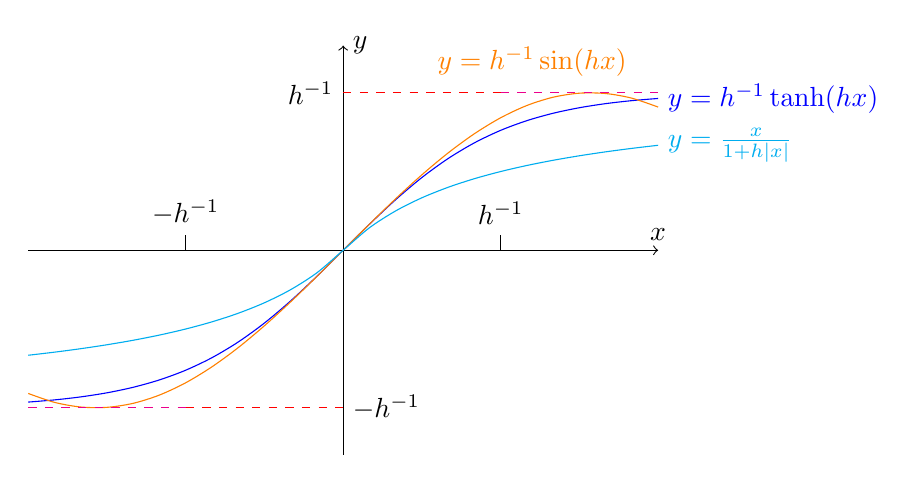
\begin{tikzpicture}[scale=0.20]
 \draw [->] (-20,0) -- (20,0) node [above] {$x$};
\draw [->] (0,-13) -- (0,13) node [right] {$y$};
%%====== 
\draw [color = blue, smooth , domain =-20:20]
  plot (\x, {10*(exp(\x/10)- exp(-\x/10))/(exp(\x/10)+ exp(-\x/10))})   node[right] {$y=h^{-1}\tanh(h x)$};
  
 \draw[color=orange, smooth, domain =-20:20]
 plot (\x, {10*sin(\x/10 r)})   node at (12,12) %node[right] 
 {$y=h^{-1}\sin(h x)$};

  \draw [ color = cyan, smooth , domain =-20:20]
  plot (\x, {\x/(1 + (abs(\x)/10})   node[right] {$y=\frac{x}{1+h|x|}$};
  
%\draw [ color =red , smooth , domain =-13:13]
%  plot (\x, {\x})   node[right] {$y =x$};
 %%===================
%  \draw [ color =magenta, smooth, thick , domain =-10:10]
 % plot (\x, {\x}); 
  
  \draw [ color =red , dashed , domain =0:10]  plot (\x, 10) ;
  
  \draw [ color =magenta , dashed, domain =10:20]
  plot (\x, 10) ;

  \draw [ color =magenta, dashed, domain =-20:-10]
plot (\x, -10) ;

    \draw [ color =red, dashed , domain =-10:0]
  plot (\x, -10) ;

%%===================
  \draw [solid] (-10,0.0) -- (-10,1)  node[above] {$-h^{-1}$};
  %
  \draw [solid](10,0) -- (10,1) node[above] {$h^{-1}$};
  
  \draw (0,-10) node[right] {$-h^{-1}$};
  \draw (0,10) node[left] {$h^{-1}$};
\end{tikzpicture}
\captionof{figure}{Several choices for the operators $\mathcal{T}_i$, $i=1,2$.}
\label{fig:sketch-popu-exam-moment-bound}
\end{center}
Also, we mention that Assumption \ref{a:euler_operator_t12} just provides sufficient conditions used to derive the moment bounds of the numerical approximations. 
%Once the moment bounds of numerical approximations are available, it is not necessary for the considered methods to satisfy all the conditions in Assumption \ref{a:euler_operator_t12}. 
We present in Subsection \ref{s:example_mod_euler} some examples of modified Euler methods fulfilling Assumption \ref{a:euler_operator_t12}. In the literature, there are numerical methods that do not satisfy the condition \textit{(H1)} in Assumption \ref{a:euler_operator_t12}, whose moment boundedness can be derived in a different way (see Example \ref{ex:fully-tamed-Euler-scheme} below quoted from \cite{Neelima20}).
%Furthermore, it's worth noting that assumption \textit{(H2')} serves as an alternative to \textit{(H2)}. Satisfaction of either one of them with \textit{(H1)} results in achieving moment boundedness of the numerical approximations.

\subsection{Examples of modified Euler approximations}
\label{s:example_mod_euler}

The following are some examples of modified Euler type methods \eqref{eq:modified_euler_scheme}, where $\mathcal T_{1}$ and $\mathcal T_{2}$ are explicitly given.

\begin{exmp}[Drift-tamed Euler (DTE) \cite{Reis22}, \cite{Liu23}]
\label{ex:drift-tamed-Euler-scheme}
In \cite{Reis22}(\cite{Liu23}), the diffusion coefficient $\sigma$ is assumed to be globally Lipschitz continuous (or H\"older continuous). In their setting, the diffusion coefficient $\sigma$ does not need to be tamed, and a drift-tamed Euler method was introduced, where
\begin{equation}
\label{eq:numerical_approximation_DTE}
\mathcal T_{1}(x, h) = \frac{x}{1+h^{\lambda}|x| }, \quad \mathcal T_{2}(x, h) = x, \quad 0 < \lambda \leq \frac{1}{2}.
\end{equation} 
\end{exmp}

In this work, we propose three new modified Euler methods as follows.

\begin{exmp}[Modified Euler method (ME)] 
\label{ex:modified-Euler-scheme}
We propose a modified Euler method, where the operators $\mathcal T_{1}$ and $\mathcal T_{2}$ are given by
\begin{equation}
\label{eq:numerical_approximation_MES}
\mathcal T_{1}(x, h) = \frac{x}{1+h|x|^2 }, \quad  \mathcal T_{2}(x, h) = \frac{x}{1+h|x|^2 }.
\end{equation}
It is straightforward to verify that the conditions \textit{(H1)} and \textit{(H2)} in Assumption \ref{a:euler_operator_t12} are satisfied with $r_1 \in (0,1]$ and $r_2 = 3$. 
%Moreover, from assumption \textit{(A2)} in Assumption \ref{a:assumption_1_existence}, we know that operators in \eqref{eq:numerical_approximation_MES} satisfy \textit{(H2')}.
\end{exmp}

\begin{exmp}[tanh Euler method (TE)] 
\label{ex:tanh-Euler-scheme}
We introduce a $\tanh$ Euler method, where the operators $\mathcal T_{1}$ and $\mathcal T_{2}$ are as follows:
\begin{equation}
\label{eq:numerical_approximation_TES}
\mathcal T_{1}(x, h) = \frac{1}{h^{\alpha}} \tanh(h^{\alpha} x), \quad  \mathcal T_{2}(x, h) = \frac{1}{h^{\alpha}} \tanh(h^{\alpha} x),
\end{equation}
for some $\alpha \in (0, 3/2)$. The conditions \textit{(H1)} and \textit{(H2)} in Assumption \ref{a:euler_operator_t12} are satisfied when we choose $r_1 \in (0, \alpha]$ and $r_2 = 2$. %Note that, the assumption \textit{(H2')} in Assumption \ref{a:euler_operator_t12} may not hold in this example.
\end{exmp}
In a similar way, we propose the sin Euler method as follows.
\begin{exmp}[sin Euler method (SE)] 
\label{ex:sin-Euler-scheme}
In the sin Euler method, the operators $\mathcal T_{1}$ and $\mathcal T_{2}$ are defined by
\begin{equation}
\label{eq:numerical_approximation_SES}
\mathcal T_{1}(x, h) = \frac{1}{h^{\alpha}} \sin(h^{\alpha} x), \quad \mathcal T_{2}(x, h) = \frac{1}{h^{\alpha}} \sin(h^{\alpha} x),
\end{equation}
for some $\alpha \in (0, 3/2)$. The conditions \textit{(H1)} and \textit{(H2)} in Assumption \ref{a:euler_operator_t12} are  fulfilled with $r_1 \in (0, \alpha)$ and $r_2 = 2$. %Likewise, in this case, \textit{(H2')} from Assumption \ref{a:euler_operator_t12} may not be satisfied.
\end{exmp}

Next, we provide tamed Euler type methods that do not satisfy Assumption \ref{a:euler_operator_t12}, but the moment boundedness and strong convergence rates of the numerical solutions have be obtained in the literature \cite{Neelima20}. 

\begin{exmp}[Fully-tamed Euler method (FTE) \cite{Neelima20}]
\label{ex:fully-tamed-Euler-scheme}
The author of \cite{Neelima20} proposed a drift-diffusion fully tamed Euler method, where 
$ \mathcal T_1, 
\mathcal T_2$ are given by
\begin{equation}
\label{eq:numerical_approximation_FTE}
\mathcal T_{1}( b(t, x, \mu), h) = 
\frac{ b(t, x, \mu)}{1+h^{\frac{1}{2}}|x|^{4\rho} }, \quad \mathcal T_{2}(\sigma_r(t, x, \mu), h) 
= \frac{ \sigma_r(t, x, \mu)}
{1+h^{\frac{1}{2}}|x|^{4 \rho} }.
\end{equation} 
Here $\rho$ comes from the growth condition (A6) of the drift $b$ below. It is not difficult to check that the mappings  $\mathcal T_1, 
\mathcal T_2$ do not obey \textit{(H1)} in Assumption \ref{a:euler_operator_t12}, but satisfy 
\begin{equation*}
\left\vert  \mathcal T_{1}( b(t, x, \mu), h) \right\vert \leq \min \big\{L h^{-\frac14}(1+|x|)+\mathcal W_2 (\mu, \delta_0), |b(t, x, \mu)| \big\}
\end{equation*} 
and
\begin{equation*}
\left\vert  \mathcal T_{2}( \sigma_r(t, x, \mu), h) \right\vert \leq \min \big\{  L h^{-\frac18}(1+|x|)+\mathcal W_2 (\mu, \delta_0), |\sigma_r(t, x, \mu)| \big\}.
\end{equation*} 
%The boundedness of the moments for the above tamed Euler method is given by (29) in \cite{Neelima20}.
\end{exmp}
%
\iffalse
\begin{exmp}[Dissipative tamed Euler  (DTE) \cite{neufeld2025non-asymptotic}]
In \cite{neufeld2025non-asymptotic}, the diffusion coefficient $\sigma$ is 
\begin{equation*}
\mathcal T_{1}( b(t, x, \mu), h) = 
\frac{ b(t, x, \mu)}{(1+h|x|^{4\rho})^{1/2} }, \quad \mathcal T_{2}(x, h) = x.
\end{equation*} 
\end{exmp}
\fi

\subsection{Boundedness of moments of modified Euler approximations}
\label{sub:bound-moment-modi-method}

As demonstrated in \cite{Higham07}, \cite{Hutzen11}, \cite{Matting02}, \cite{Mils05}, it has been established that the numerical approximation generated by the Euler-Maruyama method lacks finite moments, which is of paramount significance for achieving convergence toward the desired system of interacting particles. Subsequently, we establish that the modified Euler numerical approximations, as defined by \eqref{eq:modified_euler_scheme}, possess bounded high-order moments.


In the following, we give some assumptions on the regularity of the coefficients in MV-SDEs to establish the moment boundedness  and the convergence rate of modified Euler approximations.

\begin{assum}
\label{a:euler_coefficient_b_sigma}
\begin{enumerate}
    \item[(A5)] For some $p_1 > 1$, there exists a constant $L > 0$ such that
    \begin{equation*}
    2 \lan x - y, b(t, x, \mu) - b(t, y, \nu) \ran + (2 p_1 - 1) \|\sigma(t, x, \mu) - \sigma(t, y, \nu) \|^2 \leq L \left(|x-y|^2 + \mathcal W_2^2 (\mu, \nu) \right)
    \end{equation*}
    for all $t \in [0, T], x, y \in \R^d$ and $\mu, \nu \in \mathcal P_2(\R^d)$.
    \vspace{4pt}
    
    \item[(A6)] There exist constants $L > 0$ and $\rho > 0$ such that
    \begin{equation*}
    |b(t, x, \mu) - b(t, y, \nu) | \leq L \left( \left( 1 + |x|^{2 \rho} + |y|^{2\rho} \right) |x - y|\right) + L \mathcal W_2 (\mu, \nu)
    \end{equation*}
    for all $t \in [0, T], x, y \in \R^d$ and $\mu, \nu \in \mathcal P_2(\R^d)$.
    \vspace{4pt}
    
    \item[(A7)] There exist a constant $L > 0$ such that
    \begin{equation*}
    |b(t, x, \mu) - b(s, x, \mu) | + \|\sigma(t, x, \mu) - \sigma(s, x, \mu) \| \leq L |t - s|^{\frac{1}{2}}
    \end{equation*}
    for all $t, s \in [0, T], x \in \R^d$ and $\mu \in \mathcal P_2(\R^d)$.
\end{enumerate}
\end{assum}

\begin{rem}
We mention that, assumption (A5) is stronger than the assumption (A3) since $2 p_1 - 1 > 1$. From assumptions (A5) and (A6), it follows that there exists a constant $K := K(L) > 0$
such that
\begin{equation*}
\|\sigma(t, x, \mu) - \sigma(t, y, v)\| \leq K  \left( \left(1+ |x|^{\rho} + |y|^{\rho} \right)|x-y| + \mathcal W_{2} (\mu, \nu) \right)
\end{equation*}
for all $t \in[0, T], x, y \in \mathbb{R}^{d}$, and $\mu, \nu \in \mathcal P_{2}(\mathbb{R}^{d})$.

Moreover, due to assumptions (A2), (A6) and (A7), there exists a constant $K:= K(L, T) > 0$ such that
\begin{equation}
\label{eq:growth_condition_b}
|b(t, x, \mu)| \leq K \left(1+|x|^{2 \rho+1} + \mathcal W_{2} \left(\mu, \delta_{0} \right) \right)
\end{equation}
and
\begin{equation}
\label{eq:growth_condition_sigma}
\|\sigma(t, x, \mu)\| \leq K \left( 1 + |x|^{\rho + 1} + \mathcal W_{2} \left(\mu, \delta_{0} \right) \right)
\end{equation}
for all $t \in [0, T], x \in \mathbb{R}^{d}$ and $\mu \in \mathcal  P_{2} (\mathbb{R}^{d})$. Note that, \eqref{eq:growth_condition_b} and \eqref{eq:growth_condition_sigma} provide the growth condition for the coefficients $b$ and $\sigma$, respectively.
\end{rem}

Also, we mention that, in the above settings, the drift and diffusion coefficients of the MV-SDEs are assumed to be $\mathcal{W}_2$-Lipschitz with respect to the measure component.
%
The following moment bound result, motivated by \cite{zhao2024one}, is essential for establishing the subsequent strong convergence result.
\begin{lem}
\label{l:moment_bound_euler_discrete_time}
Suppose assumptions (A1), (A2), (A6), (A7), (H1), (H2) hold. Then, for all $k = 0, 1, \dots, n$, there exists $\beta > 1$ and $K > 0$ independent of $n$  and $h$ such that
\begin{equation}
\label{eq:moment_boundness}
\sup_{i \in \{1, 2, \dots, N\}} \mathbb E \Big[ \Big\vert X_{k}^{i, N, n} \Big\vert^{2p} \Big] \leq K \big(1  + \mathbb E [ |X_0|^{2 p \beta}] \big), \quad \forall p \in \Big[1, \frac{2 \bar p - \mathcal G}{2 + 4 \mathcal G} \Big],
\end{equation}
where
\begin{equation}
\label{eq:constant_G}
\mathcal G := \mathcal G(\rho, r_1, r_2) = \max \Big\{6 \rho, \frac{(2 \rho + 1) r_2 - 1}{r_1} \Big\}
\end{equation}
with $\rho > 0$ from (A6) and $r_1, r_2 > 0$ from (H2), and $\bar{p}$ satisfies $p_0 \geq \bar{p} \geq 1 + \frac{5}{2} \mathcal G$.
\end{lem} 
The proof of this lemma can be found in Appendix \ref{appen:proof-moment-bound-modi-method}.
%
\begin{rem}
The boundedness of the moments of existing tamed numerical methods for MV-SDEs, such as those studied in \cite{Kumar22}, \cite{Neelima20}, was obtained based on an essential use of the following coercivity condition:
%The boundedness of the moments for commonly used tamed numerical methods, such as those studied in \cite{Kumar22}, \cite{Neelima20}, and the truncated method analyzed in \cite{guo2024convergence}, can be established under an alternative one-sided Lipschitz condition. Specifically, there exists a constant $L > 0$ such that
    \begin{equation}
    \label{eq:fra-mono-con-method}
    2 \lan x,  b_h(t, x, \mu)  \ran + (2 p_0 - 1) \big\| \sigma_h  (t, x, \mu)  \big\|^2 \leq L \left( 1 + |x|^2 + \mathcal W_2^2 (\mu, \delta_0) \right)
    \end{equation}
    for all $t \in [0, T], x \in \R^d$ and $\mu \in \mathcal P_2(\R^d)$. 
Here $b_h, \sigma_h$ are certain taming modifications of the drift and diffusion coefficients $b, \sigma$.
However, the modified Euler, tanh Euler and sin Euler methods proposed in Examples \ref{ex:modified-Euler-scheme}, \ref{ex:tanh-Euler-scheme}, \ref{ex:sin-Euler-scheme} fail to satisfy the condition \eqref{eq:fra-mono-con-method}. By formulating a different framework, here we employ new and different techniques to establish the desired moment bounds for these novel methods.
\end{rem}
%%%%%%%%%%%%%%%%%%%%%%%%%%%%%%
%
\iffalse
\begin{lem}
\label{lem:Euler_scheme_mom_bound_one_side}
Under the same conditions as Lemma \ref{l:moment_bound_euler_discrete_time}, we consider a modified assumption (H2') in Assumption \ref{a:euler_operator_t12} in place of (H2). Then, for all $n \in \mathbb N$ and $k = 0, 1, \dots, n$, there exist $K > 0$ and $\beta > 1$ independent of $h$ and $n$ such that 
\begin{equation}
\label{eq:balan_euler_mom_one_side}
\sup_{i \in \{1, 2, \dots, N\}} \mathbb E \left[ \left\vert X_{k}^{i, N, n} \right\vert^{2p} \right] \leq K \left(1  + \mathbb E \left[ |X_0|^{2 p \beta}  \right] \right)
\end{equation}
for all $p \in \left[1, \frac{2 \bar p - \mathcal G}{2 + 4 \mathcal G} \right]$, where $\mathcal {G} := \mathcal {G}(\rho) = 6 \rho$ with $\rho > 0$ from (A6), and \textcolor{cyan}{$\bar{p}$ is a constant satisfying $p_0 \geq \bar{p} \geq 1 + \frac{5}{2} \mathcal{G}$.}
\end{lem}
\fi
%%%%%%%%%%%%%

\section{Strong convergence rate of modified Euler approximations}
\label{s:convergence_rate}

We prove the strong convergence rate of the modified Euler approximation \eqref{eq:modified_euler_scheme} in this section. Firstly, we provide a continuous-time version of modified Euler approximations for \eqref{eq:N_particle_system}. Let $\kappa_n(t) = \frac{\lfloor nt \rfloor}{n} = \sup \{s \in \{t_0, t_1, \dots, t_n\}, s \leq t\}$ for all $t \in [0, T]$. The modified Euler approximation in continuous time is given by
\begin{equation}
\label{eq:modified_euler_scheme_continuous_time}
\begin{aligned}
& X_{t}^{i, N, n} = X_0^i + \int_0^t \mathcal T_1 \left(b \left(\kappa_n(s), X_{\kappa_n(s)}^{i, N, n}, \mu_{\kappa_n(s)}^{X, N, n} \right), h \right) ds \\
& \hspace{0.8in} + \sum_{r = 1}^{m} \int_0^t \mathcal T_2 \left(\sigma_r \left(\kappa_n(s), X_{\kappa_n(s)}^{i, N, n}, \mu_{\kappa_n(s)}^{X, N, n} \right), h \right) dW_{r}^{i} (s)
\end{aligned}
\end{equation}
for all $t \in [0, T]$ and $i = 1, 2, \dots, N$.

Before proceeding with the proof of the rate of convergence of the modified Euler approximation \eqref{eq:modified_euler_scheme_continuous_time}, we establish some lemmas in what follows.

The following lemma provides an estimation between $X_t^{i, N, n}$ and $X_{\kappa_n(t)}^{i, N, n}$.

\begin{lem}
\label{l:difference_of_euler_numerical_scheme}
Under the same conditions of Lemma \ref{l:moment_bound_euler_discrete_time}, for all $i \in \{1,2, \dots, N\}$, $t \in[0, T]$ and $n$, $N \in \mathbb{N}$, we have the following inequality
$$
\mathbb{E} \Big[\left|X_{t}^{i, N, n} - X_{\kappa_n(t)}^{i, N, n} \right|^{2 p} \Big] \leq K h^{p}, \quad \forall p \in \Big[1, \frac{2 \bar p - \mathcal G}{(2 \rho + 1)(2 + 4 \mathcal G)} \Big],
$$
where $\mathcal G$ is given in \eqref{eq:constant_G} and $\bar{p}$ is a constant satisfying $p_0 \geq \bar{p} \geq (4 \rho + \frac{5}{2}) \mathcal G + 2 \rho + 1$. 
\end{lem}
\textit{Proof.}
Applying H\"older's inequality and the Burkholder-Davis-Gundy inequality, we have that for all $t \in [0, T]$,
\begin{equation*}
\begin{aligned}
& \mathbb{E}\left[\left|X_{t}^{i, N, n} - X_{\kappa_{n}(t)}^{i, N, n} \right|^{2 p} \right] \\
\leq \ & K \left(t - \kappa_{n}(t) \right)^{2 p - 1} \mathbb{E} \left[\int_{\kappa_{n}(t)}^{t} \left|\mathcal T_{1} \left(b \left(\kappa_{n}(s), X_{\kappa_{n}(s)}^{i, N, n}, \mu_{\kappa_{n}(s)}^{X, N, n}\right), h\right)\right|^{2 p} d s\right] \\
& \hspace{0.2in} + K \mathbb{E} \left[\left|\sum_{r=1}^{m} \int_{\kappa_{n}(t)}^{t} \mathcal T_{2}^{2} \left(\sigma_{r}\left(\kappa_{n}(s), X_{\kappa_{n}(s)}^{i, N, n}, \mu_{\kappa_{n}(s)}^{X, N, n} \right), h \right) d s \right|^{p} \right] \\
\leq \ & K h^{2 p - 1} \mathbb{E} \left[\int_{\kappa_{n}(t)}^{t} \left|\mathcal T_{1} \left( b \left(\kappa_{n}(s), X_{\kappa_{n}(s)}^{i, N, n}, \mu_{\kappa_{n}(s)}^{X, N, n}\right), h \right) \right|^{2 p} d s \right] \\
& \hspace{0.2in} + K h^{p - 1} \mathbb{E} \left[\sum_{r=1}^{m} \int_{\kappa_{n}(t)}^{t} \left|\mathcal T_{2} \left(\sigma_{r} \left(\kappa_{n}(s), X_{\kappa_{n}(s)}^{i, N, n}, \mu_{\kappa_{n}(s)}^{X, N, n} \right), h \right) \right|^{2 p} d s \right].
\end{aligned}
\end{equation*}
Under the assumption (\textit{H1}), and the growth condition for the coefficients $b$ and $\sigma$ in \eqref{eq:growth_condition_b} and \eqref{eq:growth_condition_sigma} respectively, it can be shown that
\begin{equation*}
\begin{aligned}
& \mathbb{E}\left[\left|X_{t}^{i, N, n} - X_{\kappa_{n}(t)}^{i, N, n} \right|^{2 p} \right] \\
\leq \ & K h^{2 p - 1} \mathbb{E} \left[\int_{\kappa_{n}(t)}^{t} \left| b \left(\kappa_{n}(s), X_{\kappa_{n}(s)}^{i, N, n}, \mu_{\kappa_{n}(s)}^{X, N, n} \right) \right|^{2 p} d s \right] \\
& \hspace{0.2in} + K h^{p - 1} \mathbb{E} \left[\sum_{r=1}^{m} \int_{\kappa_{n}(t)}^{t} \left|\sigma_{r} \left(\kappa_{n}(s), X_{\kappa_{n}(s)}^{i, N, n}, \mu_{\kappa_{n}(s)}^{X, N, n} \right) \right|^{2 p} d s \right] \\
\leq \ & K h^{2 p-1} \mathbb{E} \left[\int_{\kappa_{n}(t)}^{t} 1 + \left|X_{\kappa_{n}(s)}^{i, N, n}\right|^{2 p(2 \rho + 1)} + \left(\mathcal W_{2}^2 \left(\mu_{\kappa_{n}(s)}^{X, N, n}, \delta_{0} \right) \right)^{p} d s\right] \\
& \hspace{0.2in} + K h^{p - 1} \mathbb{E} \left[\int_{\kappa_{n}(t)}^{t} 1 + \left|X_{\kappa_{n}(s)}^{i, N, n} \right|^{2 p(\rho + 1)} + \left(\mathcal W_{2}^{2} \left(\mu_{\kappa_{n}(s)}^{X, N, n}, \delta_{0} \right) \right)^{p} d s \right].
\end{aligned}
\end{equation*}
From the identity \eqref{eq:w2_definition}, one can obtain
\begin{equation*}
\begin{aligned}
\mathbb{E}\left[\left|X_{t}^{i, N, n} - X_{\kappa_{n}(t)}^{i, N, n} \right|^{2 p} \right]
& \leq K h^{2 p}\left(1 + \sup_{s \in [\kappa_{n}(t), t]} \sup_{i \in \{1,2, \dots, N\}} \mathbb{E} \left[\left|X_{\kappa_{n}(s)}^{i, N, n} \right|^{2 p(2 \rho + 1)} \right] \right) \\
& \hspace{0.3in} + K h^{p} \left(1 + \sup_{s \in [\kappa_{n}(t), t]} \sup_{i \in \{1, 2, \dots, N\}} \mathbb{E} \left[ \left|X_{\kappa_{n}(s)}^{i, N, n} \right|^{2 p (\rho + 1)} \right] \right).
\end{aligned}
\end{equation*}
By the result of Lemma \ref{l:moment_bound_euler_discrete_time}, for all $i \in\{1,2, \dots, N\}$, $t \in[0, T]$, $n$, $N \in \mathbb N$ and $p \in [1, \frac{2 \bar p - \mathcal G}{(2 \rho + 1)(2 + 4 \mathcal G)}]$, we have
\begin{equation*}
\mathbb{E}\left[\left|X_{t}^{i, N, n} - X_{\kappa_{n}(t)}^{i, N, n} \right|^{2 p} \right] \leq K h^{p} \left(1 + \mathbb{E} \left[ \left|X_{0}\right|^{2 \beta p (2 \rho + 1)} \right] \right) \leq K h^{p},
\end{equation*}
as required.
\qed

The following lemma gives the boundedness of moments for the modified Euler approximation \eqref{eq:modified_euler_scheme_continuous_time}.

\begin{lem}
\label{l:moment_bound_euler_continuous_time}
Under the same conditions of Lemma \ref{l:moment_bound_euler_discrete_time}, there exist $\beta > 1$ and $K > 0$ independent of $n$ and $h$ such that
\begin{equation*}
\sup_{i \in \{1, 2, \dots, N\}} \sup_{t \in [0, T]} \mathbb E \left[ \left\vert X_{t}^{i, N, n} \right\vert^{2p} \right] \leq K \left(1  + \mathbb E \left[ |X_0|^{2 p \beta}  \right] \right), \quad \forall p \in \left[1, \frac{2 \bar p - \mathcal G}{(2 \rho + 1)(2 + 4 \mathcal G)} \right],
\end{equation*}
where $\mathcal G$ is given in \eqref{eq:constant_G} and $\bar{p}$ is a constant satisfying $p_0 \geq \bar{p} \geq (4 \rho + \frac{5}{2}) \mathcal G + 2 \rho + 1$.
\end{lem}
\textit{Proof.}
Applying Lemma \ref{l:moment_bound_euler_discrete_time} and Lemma \ref{l:difference_of_euler_numerical_scheme}, we obtain the desired result that
\begin{equation*}
\begin{aligned}
\sup_{i \in \{1, 2, \dots, N\}} \sup_{t \in [0, T]} \mathbb{E} \left[\left|X_{t}^{i, N, n} \right|^{2 p} \right]
& \leq \sup_{i \in \{1, 2, \dots, N\}} \sup_{t \in [0, T]} K \mathbb{E} \left[\left|X_{t}^{i, N, n} - X_{\kappa_{n}(t)}^{i, N, n} \right|^{2 p}\right] \\
& \hspace{0.5in} + \sup_{i \in \{1, 2, \dots, N\}} \sup_{t \in [0, T]} K \mathbb{E} \left[\left|X_{\kappa_{n} (t)}^{i, N, n} \right|^{2 p} \right] \\
& \leq K \left(1 + \mathbb{E} \left[\left|X_{0} \right|^{2 p \beta} \right] \right).
\end{aligned}
\end{equation*}
\qed

Next, we provide the assumptions for the proof of the convergence rate of the time-continuous approximation \eqref{eq:modified_euler_scheme_continuous_time}.

\begin{assum}
\label{a:euler_operator_t12_convergence}
\begin{enumerate}
\item[(H3)] There exist some constants $L > 0, r_2 > 0$ and $r_1, r_3 \geq \frac{1}{2}$ such that
\begin{equation*}
\left\vert \mathcal T_{1}(x, h) - x \right\vert \leq L h^{r_1} |x|^{r_2}, \quad
\left\vert \mathcal T_{2}(x, h) - x \right\vert \leq L h^{r_3} |x|^{r_2}
\end{equation*}
for all $x \in \mathbb{R}^{d}$ and $h \in (0,1)$.
\end{enumerate}
\end{assum}

Note that, in the assumption (\textit{H2}) of Assumption \ref{a:euler_operator_t12}, we only need $r_1> 0$. But in assumption (\textit{H3}) of Assumption \ref{a:euler_operator_t12_convergence}, we require that $r_1, r_3 \geq \frac{1}{2}$. Thus, the assumption \textit{(H3)} is slightly stronger than \textit{(H2)} as $h \in (0, 1)$.

%We remark that the Assumption \ref{a:euler_operator_t12_convergence} can be extended when the mappings $\mathcal{T}_{i}$ depend on some $w \in \R^d$, written as $\mathcal{T}_{i} = \mathcal{T}_{i} (x,h;w)$, \, $i=1,2$.


\begin{lem}
\label{l:estimation_difference}
Suppose the assumptions (A1), (A2), (A6), (A7), (H1), (H3) hold. Then, for all $p \in [1,\tilde{p}]$, there exists $K > 0$ independent of $n$ and $h$ such that
\begin{equation*}
\mathbb{E} \left[ \left| b \left(t, X_{t}^{i, N, n}, \mu_{t}^{X, N, n} \right) - \mathcal T_{1} \left( b \left(\kappa_{n}(t), X_{\kappa_{n}(t)}^{i, N, n}, \mu_{\kappa_{n}(t)}^{X, N, n} \right), h \right) \right|^{2 p} \right] \leq K h^{p}
\end{equation*}
and
\begin{equation*}
\sup_{r\in \{ 1, 2, \dots, m\}} \mathbb{E} \left[ \left|\sigma_{r} \left(t, X_{t}^{i, N, n}, \mu_{t}^{X, N, n}\right) - \mathcal T_{2}\left( \sigma_{r} \left(\kappa_{n}(t), X_{\kappa_{n}(t)}^{i, N, n}, \mu_{\kappa_{n}(t)}^{X, N, n} \right), h \right) \right|^{2 p} \right] \leq K h^{p},
\end{equation*} 
where 
\begin{equation}
\label{eq:constant_tilde_p}
\tilde{p} = \min \left\{\frac{2 \bar p - \mathcal G}{r_2 (2 \rho + 1) (2 + 4 \mathcal G)}, \, \frac{2 \bar p - \mathcal G}{4 \rho (2 \rho + 1)(2 + 4 \mathcal G)}, \, \frac{2 \bar p - \mathcal G}{(2 \rho + 1)(2 + 4 \mathcal G)} \right\}
\end{equation}
with $\mathcal G$ is given in \eqref{eq:constant_G} and $\bar p \leq p_0$ is a constant such that
\begin{footnotesize}
\begin{equation*}
\bar p \geq \max \left\{\left(16 \rho^2 + 8 \rho + \frac{1}{2} \right) \mathcal G + 8 \rho^2 + 4 \rho, \, \left(2 r_2 (2 \rho + 1) + \frac{1}{2} \right) \mathcal G + r_2 (2 \rho + 1), \,  \left(4 \rho + \frac{5}{2} \right) \mathcal G + 2 \rho + 1 \right\}.
\end{equation*}
\end{footnotesize}
\end{lem}

\textit{Proof.}
By Lemma \ref{l:difference_of_euler_numerical_scheme}, H\"older's inequality, (\textit{A6}), (\textit{A7}), (\textit{H3}), and the growth condition \eqref{eq:growth_condition_b}, we have 
\begin{equation*}
\begin{aligned}
& \mathbb{E} \left[ \left| b \left(t, X_{t}^{i, N, n}, \mu_{t}^{X, N, n} \right) - \mathcal T_{1} \left( b \left(\kappa_{n}(t), X_{\kappa_{n}(t)}^{i, N, n}, \mu_{\kappa_{n}(t)}^{X, N, n}\right), h \right) \right|^{2 p} \right] \\
\leq \ & K \mathbb{E} \left[ \left| b \left(t, X_{t}^{i, N, n}, \mu_{t}^{X, N, n} \right) - b \left(t, X_{\kappa_{n}(t)}^{i, N, n}, \mu_{\kappa_{n}(t)}^{X, N, n} \right) \right|^{2 p} \right. \\
& \hspace{0.3in} + \left| b \left(t, X_{\kappa_{n}(t)}^{i, N, n}, \mu_{\kappa_{n}(t)}^{X, N, n} \right) - b \left(\kappa_{n}(t), X_{\kappa_{n}(t)}^{i, N, n}, \mu_{\kappa_{n}(t)}^{X, N, n} \right) \right|^{2 p} \\
& \hspace{0.3in} + \left. \left| b \left(\kappa_{n}(t), X_{\kappa_{n}(t)}^{i, N, n}, \mu_{\kappa_{n}(t)}^{X, N, n} \right) - \mathcal T_{1} \left( b \left(\kappa_{n}(t), X_{\kappa_{n}(t)}^{i, N, n}, \mu_{\kappa_{n}(t)}^{X, N, n} \right), h \right) \right|^{2 p} \right] \\
\leq \ & K \mathbb{E} \bigg[ \left(1 + \left|X_{t}^{i, N, n} \right|^{2 \rho} + \left|X_{\kappa_{n}(t)}^{i, N, n} \right|^{2 \rho} \right)^{2 p} \left|X_{t}^{i, N, n} - X_{\kappa_{n}(t)}^{i, N, n} \right|^{2p} \\
& \hspace{0.3in} + \mathcal W_{2}^{2p} \left(\mu_{t}^{X, N, n}, \mu_{\kappa_{n}(t)}^{X, N, n} \right) + \left|t - \kappa_{n}(t) \right|^{p} + h^{2 p r_{1}} \left|b \left(\kappa_{n}(t), X_{\kappa_{n}(t)}^{i, N, n}, \mu_{\kappa_{n}(t)}^{X, N, n} \right) \right|^{2 p r_{2}}\bigg] \\
\iffalse
\leq \ & K h^p \mathbb{E} \left[  \left(1 + \left|X_{t}^{i, N, n} \right|^{8p \rho} + \left|X_{\kappa_{n}(t)}^{i, N, n} \right|^{8p \rho} \right) \right] + K \mathbb E \left[ \left(\frac{1}{N} \sum_{i=1}^{N}\left|X_{t}^{i, N, n} - X_{\kappa_{n}(t)}^{i, N, n} \right|^{2} \right)^{p} \right] \\
& \hspace{0.3in} + K h^{p} + K h^{2 p r_{1}} \mathbb E \left[ \left(1 + \left|X_{\kappa_{n}(t)}^{i, N, n} \right|^{2 \rho + 1} + \mathcal W_{2} \left(\mu_{\kappa_{n}(t)}^{X, N, n},  \delta_{0} \right) \right)^{2 p r_{2}} \right] \\
\fi
\leq \ & K h^p \mathbb{E} \left[\left(1 + \left|X_{t}^{i, N, n} \right|^{8p \rho} + \left|X_{\kappa_{n}(t)}^{i, N, n} \right|^{8p \rho} \right)  \right] + K \sup_{i \in \{1, 2, \dots, N\}} \mathbb{E} \left[ \left| X_{t}^{i, N, n} - X_{\kappa_{n}(t)}^{i, N, n} \right|^{2 p} \right] + K h^{p} \\
& \hspace{0.3in} + K h^{2 p r_{1}} \mathbb{E} \left[1 + \left|X_{\kappa_{n}(t)}^{i, N, n} \right|^{2 p r_{2}(2 \rho + 1)} + \mathcal W_{2}^{2 p r_2} \left(\mu_{\kappa_{n}(s)}^{X, N, n}, \delta_{0} \right) \right]
\end{aligned}
\end{equation*}
since
\begin{equation*}
\mathcal W_{2}^{2} \left(\mu_{t}^{X, N, n}, \mu_{\kappa_{n}(t)}^{X, N, n} \right) \leq \frac{1}{N} \sum_{i=1}^{N}\left|X_{t}^{i, N, n} - X_{\kappa_{n}(t)}^{i, N, n} \right|^{2} \leq \sup_{i \in \{1, 2, \dots, N\}} \left|X_{t}^{i, N, n} - X_{\kappa_{n}(t)}^{i, N, n} \right|^{2}.
\end{equation*}
Then, Lemmas \ref{l:moment_bound_euler_discrete_time}, \ref{l:difference_of_euler_numerical_scheme} and \ref{l:moment_bound_euler_continuous_time} together show that
\begin{equation*}
\begin{aligned}
& \mathbb{E} \left[ \left| b \left(t, X_{t}^{i, N, n}, \mu_{t}^{X, N, n} \right) - \mathcal T_{1} \left( b \left(\kappa_{n}(t), X_{\kappa_{n}(t)}^{i, N, n}, \mu_{\kappa_{n}(t)}^{X, N, n}\right), h \right) \right|^{2 p} \right] \\
\leq \ &  K h^{p} \left(1 + \mathbb{E} \left[ \left|X_{0} \right|^{8 p \rho \beta} \right] \right) + K h^{p} + K h^{2 p r_{1}} \left(1 + \mathbb{E} \left[\left|X_{0} \right|^{2 p \beta r_{2}(2 \rho + 1)} \right] \right) \\
& \hspace{0.3in} + K h^{2 p r_{1}} \mathbb{E} \left[\left(\frac{1}{N} \sum_{i=1}^{N} \left|X_{\kappa_{n}(s)}^{i, N, n} \right|^{2} \right)^{p r_{2}} \right] \\
\leq \ & K h^{p}
\end{aligned}
\end{equation*}
since $r_1 \geq \frac{1}{2}$. The proof is completed by performing a similar calculation for $\sigma_r$ for all $r = 1, 2, \dots, m$ with $r_2 \geq \frac{1}{2}$.
\qed

Now, we are ready to prove the strong convergence rate of order $\frac{1}{2}$ for the modified Euler approximation \eqref{eq:modified_euler_scheme_continuous_time} in the $L^p$ sense. 
%The following Theorem is the main result of this section.

\begin{thm}
\label{t:convergence_rate_euler}
Suppose assumptions (A1), (A2), (A5), (A6), (A7), (H1), (H3) are satisfied. Then, the modified Euler approximation \eqref{eq:modified_euler_scheme_continuous_time} converges to the solution of the interacting particle system \eqref{eq:N_particle_system} in a strong sense with $L^p$ convergence rate given by
$$
\sup_{i \in \{1, 2, \dots, N\}} \sup_{t \in [0, T]} \mathbb{E} \left[ \left|X_{t}^{i, N} -X_{t}^{i, N, n} \right|^{2 p} \right] \leq K h^{p}
$$
for all $1 \leq p \leq \min \{\frac{1}{2} p_{1} + \frac{1}{4}, \tilde{p} \}$, where $p_1$ comes from assumption \textit{(A5)}, $\tilde{p}$ is given by \eqref{eq:constant_tilde_p} and $K > 0$ does not depend on $n, N \in \mathbb N$.
\end{thm}
\textit{Proof.}
From \eqref{eq:N_particle_system}, \eqref{eq:modified_euler_scheme_continuous_time}, and Ito's formula, it follows that
\begin{equation*}
\begin{aligned}
& \left|X_{t}^{i, N} - X_{t}^{i, N, n} \right|^{2 p} \\
= \ & 2 p \int_{0}^{t} \left|X_{s}^{i, N} - X_{s}^{i, N, n} \right|^{2 p - 2} \left\langle X_{s}^{i, N} - X_{s}^{i, N, n}, b \left(s, X_{s}^{i, N}, \mu_{s}^{X, N} \right) - \mathcal T_{1} \left(b \left(\kappa_{n}(s), X_{\kappa_{n}(s)}^{i, N, n}, \mu_{\kappa_{n}(s)}^{X, N, n} \right), h \right) \right\rangle d s \\
& \hspace{0.1in} + 2 p \int_{0}^{t} \left|X_{s}^{i, N} - X_{s}^{i, N, n} \right|^{2 p - 2} \sum_{r=1}^{m} \left\langle X_{s}^{i, N} - X_{s}^{i, N, n}, \sigma_{r} \left(s, X_{s}^{i, N}, \mu_{s}^{X, N} \right) - \mathcal T_{2} \left(\sigma_{r} \left(\kappa_{n}(s), X_{\kappa_{n}(s)}^{i, N, n}, \mu_{\kappa_{n}(s)}^{X, N, n} \right) , h \right)  \right\rangle d W_{r}^{i}(s) \\
& \hspace{0.1in} +  p (2 p - 1) \int_{0}^{t} \left|X_{s}^{i, N} - X_{s}^{i, N, n} \right|^{2 p-2} \sum_{r=1}^{m}\left|\sigma_{r} \left(s, X_{s}^{i, N}, \mu_{s}^{X, N} \right) - \mathcal T_{2} \left(\sigma_{r} \left(\kappa_{n}(s), X_{\kappa_{n}(s)}^{i, N, n}, \mu_{\kappa_{n}(s)}^{X, N, n} \right) , h \right) \right|^{2} d s.
\end{aligned}
\end{equation*}
Taking expectation and applying the Cauchy–Schwarz inequality, we have
\begin{equation*}
\begin{aligned}
& \mathbb{E} \left[\left|X_{t}^{i, N} - X_{t}^{i, N, n} \right|^{2 p} \right] \\ 
\leq \ & p \mathbb{E} \left[\int_{0}^{t} \left|X_{s}^{i, N} - X_{s}^{i, N, n} \right|^{2p - 2} \Big\{ \Big\langle 2 \left(X_{s}^{i, N} - X_{s}^{i, N, n} \right), b \left(s, X_{s}^{i, N}, \mu_{s}^{X, N} \right) - b \left(s, X_{s}^{i, N, n}, \mu_{s}^{X, N, n} \right) \right.  \\
& \hspace{0.2in} + b \left(s, X_{s}^{i, N, n}, \mu_{s}^{X, N, n} \right) - \mathcal T_{1} \left(b \left(\kappa_{n}(s), X_{\kappa_{n}(s)}^{i, N, n}, \mu_{\kappa_{n}(s)}^{X, N, n} \right), h \right)\Big\rangle \\
& \hspace{0.2in} + (2 p - 1) \sum_{r=1}^{m} \Big| \sigma_{r} \left(s, X_{s}^{i, N}, \mu_{s}^{X, N} \right) - \sigma_{r} \left(s, X_{s}^{i, N, n}, \mu_{s}^{X, N, n} \right) \\
& \hspace{0.2in} \left. \left. + \sigma_{r} \left(s, X_{s}^{i, N, n}, \mu_{s}^{X, N, n} \right) - \mathcal T_{2} \left(\sigma_{r} \left(\kappa_{n}(s), X_{\kappa_{n}(s)}^{i, N, n}, \mu_{\kappa_{n}(s)}^{X, N, n} \right) , h \right) \Big|^2 \right. \Big\} ds \right].
\end{aligned}
\end{equation*}
Noting $p \leq \frac{1}{2} p_1 + \frac{1}{4}$, we derive that
\begin{equation*}
\begin{aligned}
& \mathbb{E} \left[\left|X_{t}^{i, N} - X_{t}^{i, N, n} \right|^{2 p} \right] \\
\leq \ & p \mathbb{E} \bigg[\int_{0}^{t} \left|X_{s}^{i, N} - X_{s}^{i, N, n} \right|^{2p - 2} \Big\{ \left\langle 2 \left(X_{s}^{i, N} - X_{s}^{i, N, n} \right), b \left(s, X_{s}^{i, N}, \mu_{s}^{X, N} \right) - b \left(s, X_{s}^{i, N, n}, \mu_{s}^{X, N, n} \right) \right\rangle \\
& \hspace{0.1in} + (2 p_1 - 1) \sum_{r=1}^{m} \left| \sigma_{r} \left(s, X_{s}^{i, N}, \mu_{s}^{X, N} \right) - \sigma_{r} \left(s, X_{s}^{i, N, n}, \mu_{s}^{X, N, n} \right) \right|^2 \Big\} ds \bigg] \\
& \hspace{0.1in} + K \mathbb{E} \left[\int_{0}^{t} \left|X_{s}^{i, N} - X_{s}^{i, N, n} \right|^{2p - 2} \left\langle \left(X_{s}^{i, N} - X_{s}^{i, N, n} \right), b \left(s, X_{s}^{i, N, n}, \mu_{s}^{X, N, n} \right) - \mathcal T_{1} \left(b \left(\kappa_{n}(s), X_{\kappa_{n}(s)}^{i, N, n}, \mu_{\kappa_{n}(s)}^{X, N, n} \right), h \right) \right\rangle ds \right] \\
& \hspace{0.1in} + K \mathbb{E} \bigg[\int_{0}^{t} \left|X_{s}^{i, N} - X_{s}^{i, N, n} \right|^{2p - 2} \sum_{r=1}^{m} \left| \sigma_{r} \left(s, X_{s}^{i, N, n}, \mu_{s}^{X, N, n} \right) - \mathcal T_{2} \left(\sigma_{r} \left(\kappa_{n}(s), X_{\kappa_{n}(s)}^{i, N, n}, \mu_{\kappa_{n}(s)}^{X, N, n} \right) , h \right) \right|^2  ds \bigg]
\end{aligned}
\end{equation*}
for all $t \in[0, T], i \in \{1,2, \dots, N\}$ and $n, N \in \mathbb N$. By using the Cauchy–Schwarz inequality, Young's inequality, and Assumption (\textit{A5}), one can obtain
\begin{equation*}
\begin{aligned}
& \mathbb{E} \left[\left|X_{t}^{i, N} - X_{t}^{i, N, n} \right|^{2 p} \right] \\
\leq \ &  K \mathbb{E} \left[ \int_{0}^{t} \left|X_{s}^{i, N} - X_{s}^{i, N, n} \right|^{2 p} d s \right] + K \mathbb{E} \left[\int_{0}^{t} \mathcal W_{2}^{2 p} \left(\mu_{s}^{X, N}, \mu_{s}^{X, N, n} \right) d s \right] \\
& \hspace{0.2in} + K \mathbb{E} \left[ \int_{0}^{t} \left| b \left(s, X_{s}^{i, N, n}, \mu_{s}^{X, N, n} \right) - \mathcal T_{1} \left(b \left(\kappa_{n}(s), X_{\kappa_{n}(s)}^{i, N, n}, \mu_{\kappa_{n}(s)}^{X, N, n} \right), h \right) \right|^{2p} d s \right] \\
& \hspace{0.2in} + K \mathbb{E} \bigg[ \int_{0}^{t} \sum_{r=1}^{m} \left| \sigma_{r} \left(s, X_{s}^{i, N, n}, \mu_{s}^{X, N, n} \right) - \mathcal T_{2} \left(\sigma_{r} \left(\kappa_{n}(s), X_{\kappa_{n}(s)}^{i, N, n}, \mu_{\kappa_{n}(s)}^{X, N, n} \right) , h \right) \right|^{2p}  ds \bigg].
\end{aligned}
\end{equation*}
%
Lemma \ref{l:estimation_difference} along with the following estimate
$$\mathcal W_{2}^{2} \left(\mu_{s}^{X, N}, \mu_{s}^{X, N, n} \right) \leq \frac{1}{N} \sum_{i=1}^{N}\left|X_{s}^{i, N} - X_{s}^{i, N, n} \right|^{2}$$
for all $s \in [0, t]$ yields 
\begin{equation*}
\begin{aligned}
& \mathbb{E} \left[\left|X_{t}^{i, N} - X_{t}^{i, N, n} \right|^{2 p} \right] \\
\leq \ & K \mathbb{E} \left[ \int_{0}^{t} \left|X_{s}^{i, N} - X_{s}^{i, N, n} \right|^{2 p} d s \right] + K \mathbb{E} \left[\int_{0}^{t} \left(\frac{1}{N} \sum_{i=1}^{N}\left|X_{s}^{i, N} - X_{s}^{i, N, n} \right|^{2} \right)^{p} d s \right] + K \mathbb{E} \left[\int_{0}^{t} h^p  ds \right] \\
\leq \ & K \mathbb{E} \left[ \int_{0}^{t} \sup_{i \in \{1, 2, \dots, N\} }  \left|X_{s}^{i, N} - X_{s}^{i, N, n} \right|^{2 p} d s \right] + K h^p.
\end{aligned}
\end{equation*}
Therefore, the following inequality
\begin{equation*}
\sup_{i \in \{1, 2, \dots, N\} }  \sup_{r \in [0, t]} \mathbb{E} \left[\left|X_{r}^{i, N} - X_{r}^{i, N, n} \right|^{2 p} \right] \leq  K \int_{0}^{t} \sup_{i \in \{1, 2, \dots, N\} } \sup_{r \in [0, s]} \mathbb{E} \left[ \left|X_{r}^{i, N} - X_{r}^{i, N, n} \right|^{2 p} \right] d s + K h^p
\end{equation*}
holds for all $t \in [0, T]$, $i \in \{1, 2, \dots, N\}$ and $n, N \in \mathbb N$. The application of Gr\"onwall's inequality implies
\begin{equation*}
\sup_{i \in \{1, 2, \dots, N\} }  \sup_{t \in [0, T]} \mathbb{E} \left[\left|X_{t}^{i, N} - X_{t}^{i, N, n} \right|^{2 p} \right] \leq K h^p.
\end{equation*}
The proof is thus finished.
\qed
%

\begin{dis}
\label{dis:para-value-example}
Under the assumptions of Theorem \ref{t:convergence_rate_euler}, the strong convergence rates of the modified Euler approximations \eqref{eq:modified_euler_scheme_continuous_time} can be derived, depending on the specific modifications made to the coefficients. Specifically:
\begin{itemize}
    \item For Example \ref{ex:modified-Euler-scheme}, we confirm that assumption (H3) is satisfied with $r_1 =\frac12 $, $r_2=2$, $r_3=\frac12$.
     \item For Example \ref{ex:tanh-Euler-scheme}, we demonstrate that assumption (H3) is fulfilled with $r_1 =\frac12 $, $r_2=2$, $r_3=\frac12$.
     \item For Example \ref{ex:sin-Euler-scheme}, it is clear that assumption (H3) holds with $r_1 =\frac12 $, $r_2=2$, $r_3=\frac12$.
%     \item For Example \ref{ex:fully-tamed-Euler-scheme}, we find that assumption (H3) is satisfied with $r_1 =\frac12 $, $r_2= 6 \rho + 1$, $r_3=\frac12$. Here $\rho$ is from the assumption (A6).
\end{itemize}
As a consequence of Theorem \ref{t:convergence_rate_euler}, the strong convergence rate of order $1/2$ is achieved for numerical methods defined by Examples \ref{ex:modified-Euler-scheme}, \ref{ex:tanh-Euler-scheme} and \ref{ex:sin-Euler-scheme}.   
\end{dis}

To ensure the completeness of our work, we now are ready to present the full numerical approximation errors of the modified Euler approximation \eqref{eq:modified_euler_scheme_continuous_time} to the solution of McKean-Vlasov SDE \eqref{eq:MV_SDE}. It is a straightforward result from the combination of Theorem \ref{t:convergence_rate_euler} and Proposition \ref{l:propagation_of_chaos}. 
\begin{cor}
\label{c:convergence_rate_euler}
Suppose assumptions (A1), (A2), (A3), (A4), (A5), (A6), (A7), (H1), (H3) are satisfied with $p_0 > 2$. Then, the modified Euler approach \eqref{eq:modified_euler_scheme_continuous_time} converges to the solution of McKean-Vlasov SDEs \eqref{eq:MV_SDE} in a strong sense with $L^2$ convergence rate given by
\begin{equation*}
\sup_{i \in \{1, 2, \dots, N\}} \sup_{t \in [0, T]} \mathbb{E} \left[ \left|X_{t}^{i} -X_{t}^{i, N, n} \right|^{2} \right] \leq K 
\begin{cases} 
h + N^{-\frac{1}{2}}, & d < 4, \\
h + N^{-\frac{1}{2}} \ln (N), & d = 4, \\
h + N^{-\frac{2}{d},} & d > 4,
\end{cases}
\end{equation*}
where $K > 0$ is independent of $n$ and $N \in \mathbb N$.
\end{cor}

%%%%%%%%%%%%%%%%%%%%%%%%%%%%%%%%%%%%%%%%%%%%%%%%%%%%%%%%%%%%%%%%%%%%

\section{Numerical experiments}
\label{sec:numer-results} 
Some numerical experiments are conducted to illustrate the previous theoretical findings. 
%We use the Mersenne Twister random generator with the seed $100$ in MATLAB in the following simulations. 
Newton's method is used to solve implicit algebraic equations if necessary.

We begin by considering two examples to illustrate the mean square convergence rates of the modified Euler method (ME) \eqref{eq:numerical_approximation_MES}, the tanh Euler method (TE) \eqref{eq:numerical_approximation_TES} and the sin Euler method (SE) \eqref{eq:numerical_approximation_SES}. For these examples, the coefficients satisfy Assumption 11, where both the drift and diffusion terms are non-globally Lipschitz.

To approximate the law $\mathcal L(X_{t_k})$ at each time step $t_k$ for $k = 0, 1, \dots, n$ by its empirical distribution, we apply the particle method with the number of particles $N = 100$.

As we do not know the exact solution of the considered examples, the strong convergence with respect to the number of time steps is assessed by comparing two solutions computed on a fine and coarse time grid, respectively, using the same samples of Brownian motion. The reference values of the models are computed based on a Monte Carlo method combined with the approximations and $h_{ref} =2^{-17} $. We also apply Monte Carlo method to compute the root-mean-square error (RMSE) in step size $h = \{2^{- 13}, 2^{- 13.5}, 2^{- 14}, 2^{- 14.5}, 2^{- 15}, 2^{- 15.5}, 2^{- 16}\}$ by
$$
\text{RMSE} := \sqrt{\frac{1}{N} \sum_{i = 1}^{N} \left(X_{T}^{i, N, n} - X_{T}^{i, N, n_h} \right)^2}
$$
at the terminal time $T = 1$, where $i$ refers to the $i$-th particle, and $n = T/h_{ref} = 2^{17}$ and $n_h = \lfloor T/h \rfloor$ are the corresponding time steps in the fine and coarse time grid, respectively.

\begin{figure}[htb]
\begin{minipage}{\linewidth}
\centering
\subcaptionbox{}	
{\includegraphics[width=0.42\linewidth, height=0.28\textheight]{Figures/Example_22.eps}}\quad
\subcaptionbox{}
{\includegraphics[width=0.42\linewidth, height=0.28\textheight]{Figures/Example_23.eps}}
\caption{Strong errors for Example \ref{ex:numerical_ex1_nonlinear_diff} and \ref{ex:numerical_ex2_nonlinear_diff}}
\label{fig:strong-error-non-linear-diff}
\end{minipage}
\end{figure}


\begin{exmp}
\label{ex:numerical_ex1_nonlinear_diff}
As the first test model, we consider the following McKean-Vlasov SDE
\begin{equation*}
\label{eq:non_linear_model_1}
\begin{cases}
d X_t = \left( X_t - X_t^3 + c \E[ X_t ] \right) d t + \gamma \left( 1 - X_t^2 \right) d W(t), \quad t \in (0, T], \\
X_0 = x, 
\end{cases}
\end{equation*}
with the parameter values $\gamma = 0.5$, $c = 1$, and $x = 0$. The conditions in Assumption \ref{a:euler_coefficient_b_sigma} are fulfilled with $\rho \geq 1$.
\end{exmp}
For this example, we test the RMSE of three different numerical methods ME \eqref{eq:numerical_approximation_MES}, SE \eqref{eq:numerical_approximation_SES} with $\alpha = 1/2$ and SE \eqref{eq:numerical_approximation_SES} with $\alpha = 1$. As expected, the strong convergence rates of ME \eqref{eq:numerical_approximation_MES}, SE \eqref{eq:numerical_approximation_SES} with $\alpha = 1/2$ and SE \eqref{eq:numerical_approximation_SES} with $\alpha = 1$ are close to $1/2$ from Fig. \ref{fig:strong-error-non-linear-diff} (a).
\begin{exmp}
\label{ex:numerical_ex2_nonlinear_diff}
For the second test model, we consider a McKean-Vlasov SDE in which the drift term preserves higher-order growth condition:
\begin{equation*}
\label{eq:non_linear_model_2}
\begin{cases}
d X_t = \left( 1 - X_t^5 + X_t^3 + c \E[ X_t ] \right) d t + \left(\gamma X_t^2 + 1 \right) d W(t), \quad t \in (0, T], \\
X_0 = x, 
\end{cases}
\end{equation*}
with the parameter values $c = 1$, $\gamma = 0.01$ and $x = 0$. It is clear that Assumption \ref{a:euler_coefficient_b_sigma} is 
satisfied if $\rho \geq 2$.
\end{exmp}
In Fig. \ref{fig:strong-error-non-linear-diff} (b), we reveal the RMSE of three different numerical methods ME \eqref{eq:numerical_approximation_MES}, TE \eqref{eq:numerical_approximation_TES} with $\alpha = 1/2$ and TE \eqref{eq:numerical_approximation_TES} with $\alpha = 1$ against the same step sizes on the $\log_2(\cdot)$ scale. The strong error rate is $1/2$ as expected in Theorem \ref{t:convergence_rate_euler}.

The third example features a non-globally Lipschitz drift and a global Lipschitz diffusion with respect to the state. We test the drift-tamed Euler (DTE) \eqref{eq:numerical_approximation_DTE}, the modified Euler method (ME) \eqref{eq:numerical_approximation_MES}, the tanh Euler method (TE) \eqref{eq:numerical_approximation_TES}, the sin Euler method (SE) \eqref{eq:numerical_approximation_SES} and the  fully-tamed Euler method (FTE) \eqref{eq:numerical_approximation_FTE} facilitating a comparative analysis with an alternative numerical approach, the split-step method (SSM) proposed in \cite{chen2022flexible}, \cite{chen2024euler}, and \cite{chen2023wellposedness}.

\begin{exmp}
\label{ex:linear_diff_ini_norm_distri}
We consider the double-well model considered in \cite{chen2024euler}, given by
\begin{equation*}
 \begin{cases}
d X_t = \left( -\frac54 X_t^3 + 3 X_t^2 \E[ X_t ] -3 X_t \E[ X^2_t ]+\E[ X^3_t ]\right) d t + X_t d W(t), \quad t \in (0, T], \\
X_0 \sim \mathcal{N}(\mu,\,\sigma^{2}), 
\end{cases} 
\end{equation*}
where $\mathcal{N}(\mu, \sigma^2)$ is the normal distribution with mean $\mu$ and variance $\sigma^2$. There are three stable states $\{-2,0,2\}$ for this
model \cite{tugaut2013convergence}. 
\end{exmp}

\begin{figure}
\begin{center}
\includegraphics[height=4.15cm,width=6cm]{Figures/drift-tamed-ssm-01-density.png}   
\caption{Density with $X_0 \sim \mathcal{N}(0,\,1)$}  
\label{fig:lin-diff-density-drift-ssm}
\end{center} 
\end{figure}

\begin{figure}
\begin{center}
\includegraphics[height=4.15cm, width=6cm]{./Figures/drift-tamed-ssm-33-density.png} 
\caption{Density with $X_0 \sim \mathcal{N}(3,\,9)$}  
\label{fig:lin-diff-density-drift-ssm-33}
\end{center} 
\end{figure}

\begin{figure}
\begin{center}
\includegraphics[height=4.15cm, width=6cm]{./Figures/me-te-density-01.png}    
\caption{Density with $X_0 \sim \mathcal{N}(0,\,1)$}  
\label{fig:lin-diff-density-ME-TE-01}  
\end{center} 
\end{figure}

\begin{figure}
\begin{center}
\includegraphics[height=4.15cm, width=6cm]{./Figures/me-te-density-33.png}    
\caption{Density with $X_0 \sim \mathcal{N}(3,\,9)$}  
\label{fig:lin-diff-density-ME-TE-33}  
\end{center} 
\end{figure}
%%%%%%%%%%
\begin{figure}[htb]
\begin{minipage}{\linewidth}
\centering
\subcaptionbox{}	
{\includegraphics[width=0.35\linewidth, height=0.28\textheight]{./Figures/fully-tamed-density-01.png}}\quad
\subcaptionbox{}
{\includegraphics[width=0.35\linewidth, height=0.28\textheight]{./Figures/fully-tamed-density-33.png}}
\caption{Density with $X_0 \sim \mathcal{N}(0,\,1)$(a) and $X_0 \sim \mathcal{N}(3,\,9)$(b)}
\label{fig:density-fully-tamed}
\end{minipage}
\end{figure}
%%%%%
%%%%%%%%%%
\begin{figure}[htb]
\begin{minipage}{\linewidth}
\centering
\subcaptionbox{}	
{\includegraphics[width=0.35\linewidth, height=0.30\textheight]{./Figures/SE-density-01.png}}\quad
\subcaptionbox{}
{\includegraphics[width=0.35\linewidth, height=0.30\textheight]{./Figures/SE-density-33.png}}
\caption{Density with $X_0 \sim \mathcal{N}(0,\,1)$(a) and $X_0 \sim \mathcal{N}(3,\,9)$(b)}
\label{fig:density-SE}
\end{minipage}
\end{figure}
%%%%%

Using the same setup as in \cite{chen2024euler} with $N=1000$, and computing the reference solution with a step size of $h = 10^{-4}$, Figs. \ref{fig:lin-diff-density-drift-ssm}-\ref{fig:density-SE} show density maps for DTE \eqref{eq:numerical_approximation_DTE} with $\lambda=1/2$, ME \eqref{eq:numerical_approximation_MES}, TE \eqref{eq:numerical_approximation_TES} with $\alpha = 1$, SE \eqref{eq:numerical_approximation_SES} with $\alpha = 1$, FTE \eqref{eq:numerical_approximation_FTE} and SSM. These results use a step size of $h=10^{-2}$ and are shown at times $T = 1,3,10$ for two different initial distributions $\mathcal{N}(0,\,1), \mathcal{N}(3,\,9)$. Simulated paths of these methods with the initial distribution $\mathcal{N}(3,\,9)$ are illustrated in Figs. \ref{fig:paths-val-drift-tamed}-\ref{fig:paths-value-SE}.

As noted in \cite{chen2024euler}, for large initial values (i.e., $X_0 \sim \mathcal{N}(3,\,9)$), the DTE \eqref{eq:numerical_approximation_DTE} with 
$\lambda=1/2$ produces unacceptable results (see Fig \ref{fig:lin-diff-density-drift-ssm-33}). This happens because the method \eqref{eq:numerical_approximation_DTE} becomes unstable with the stepsize $h=10^{-2}$, as clearly indicated by Fig. \ref{fig:paths-val-drift-tamed}. 
Similar phenomenon can be also detected for the SE \eqref{eq:numerical_approximation_SES} (see Fig. \ref{fig:density-SE}, \ref{fig:paths-value-SE}).
In contrast, the SSM (\cite{chen2024euler}, \cite{chen2022flexible}), ME \eqref{eq:numerical_approximation_MES}, TE \eqref{eq:numerical_approximation_TES} with $\alpha = 1$ and FTE \eqref{eq:numerical_approximation_FTE} produce acceptable results in the same setting.
Interestingly, by decreasing the stepsize to e.g.,
$h = 0.004$, the DTE \eqref{eq:numerical_approximation_DTE} with 
$\lambda=1/2$ and SE \eqref{eq:numerical_approximation_SES} with $\alpha = 1$ can be then stable and give acceptable approximations.

In terms of the density maps depicted in Figs. \ref{fig:lin-diff-density-drift-ssm}-\ref{fig:density-SE}, one can clearly observe that, the TE \eqref{eq:numerical_approximation_TES} performs most closely to the SSM and gives more reliable approximations than the other explicit methods.


\begin{figure}
\begin{center}
\includegraphics[height=4.0cm,width=6.5cm]{./Figures/dfift-tamed-unstabble-same-step.png}    % The printed column  
\caption{Paths of drift-tamed method for Example \ref{ex:linear_diff_ini_norm_distri}} 
\label{fig:paths-val-drift-tamed}
\end{center}
\end{figure}

\begin{figure}
\begin{center}
\includegraphics[height=4.0cm,width=6cm]{Figures/modified-method-stable-same-step.png}    % The printed column  
\caption{Paths of modified Euler method for Example \ref{ex:linear_diff_ini_norm_distri}}  
\label{fig:paths-val-ME}                   
\end{center}                               
\end{figure}

\begin{figure}
\begin{center}
\includegraphics[height=4.0cm,width=6cm]{Figures/tanh-stable-same-step}    % The printed column  
\caption{Paths of tanh Euler method for Example \ref{ex:linear_diff_ini_norm_distri}}  % width is 8.4 cm.
\label{fig:paths-value-TE}      
\end{center}                               
\end{figure}

\begin{figure}
\begin{center}
\includegraphics[height=4.0cm,width=6cm]{Figures/ssm-stable-same-step.png}    % The printed column  
\caption{Paths of split-step method for Example \ref{ex:linear_diff_ini_norm_distri}}  
\label{fig:paths-value-SSM}   
\end{center}                               
\end{figure}

\begin{figure}
\begin{center}
\includegraphics[height=4.0cm,width=6cm]{./Figures/fully-tamed-method-paths.png}    % The printed column  
\caption{Paths of fully-tamed Euler method for Example \ref{ex:linear_diff_ini_norm_distri}}  % width is 8.4 cm.
\label{fig:paths-value-FTE}                
\end{center}    
\end{figure}

\begin{figure}
\begin{center}
\includegraphics[height=4.0cm,width=6cm]{./Figures/SE-paths-1125.png}    % The printed column  
\caption{Paths of sin Euler method for Example \ref{ex:linear_diff_ini_norm_distri}}  % width is 8.4 cm.
\label{fig:paths-value-SE}                 
\end{center}          
\end{figure}


To sum up,
as an implicit method, the SSM method has better stability properties than the other explicit methods and can thus always produce reliable approximations even when treating  MV-SDEs with relatively large initial values and relatively large stepsize $h$. However, some explicit methods, such as the DTE \eqref{eq:numerical_approximation_DTE} and SE \eqref{eq:numerical_approximation_SES} with $\alpha = 1$, might be sensitive to the stepsize selection. Moreover, the above numerical results demonstrate that the TE \eqref{eq:numerical_approximation_TES} performs better than the other explicit methods.


\newpage

\begin{ack}                 
This work was supported by NSF grant of China (No.12471394, 12071488, 12371417) and the Postdoctoral Fellowship Program of CPSF under Grant Number GZC2024205.

We are grateful to four anonymous refrees and the associate editor for providing valuable suggestions.
\end{ack}

\bibliographystyle{plain}        % Include this if you use bibtex 
\bibliography{autosam}           % and a bib file to produce the 
                                 % bibliography (preferred). The
                                 % correct style is generated by
                                 % Elsevier at the time of printing.

%\begin{thebibliography}{99}     % Otherwise use the  
                                 % thebibliography environment.
                                 % Insert the full references here.
                                 % See a recent issue of Automatica 
                                 % for the style.


\appendix
\section{Proof of Lemma \ref{l:moment_bound_euler_discrete_time} in Section \ref{sub:bound-moment-modi-method}}
\label{appen:proof-moment-bound-modi-method}
\textit{{Proof of} Lemma \ref{l:moment_bound_euler_discrete_time}}.
In the following, we use $K$ to denote the generic constant which is independent of $n$ and $h$. Let $\mathcal R > 0$ be sufficiently large and define a sequence of decreasing subevents
$$
\Omega_{\mathcal R, k} = \left\{\omega \in \Omega : \left\vert X_{j}^{i, N, n}(\omega)\right\vert \leq \mathcal R, \, j = 0, 1, \dots, k \right\}
$$
for $k = 0,1, \dots, n$. We denote the complement of $\Omega_{\mathcal R, k}$ by $\Omega_{\mathcal R, k}^{c}$.

Firstly, we show that the boundedness of the moment is valid within a family of appropriate subevents $\left\{\Omega_{\mathcal R, k} \right\}_{k \in \{0,1, \dots, n\}}$. Note that 
\begin{equation}
\label{eq:discom_sub_event_scheme}
\begin{aligned}
& \mathbb{E} \left[\1_{\Omega_{\mathcal{R}, k+1}} \left\vert X_{k+1}^{i, N, n} \right\vert^{2 \bar p} \right] \leq \mathbb{E} \left[\1_{\Omega_{\mathcal R, k}} \left|X_{k+1}^{i, N, n}\right|^{2 \bar p}\right]  \\
= \ & \mathbb{E} \left[\1_{\Omega_{\mathcal R, k}} \left|X_{k+1}^{i, N, n} - X_{k}^{i, N, n} + X_{k}^{i, N, n} \right|^{2 \bar p} \right] \\
\leq \ & \mathbb{E} \left[\1_{\Omega_{\mathcal R, k}} \left|X_{k}^{i, N, n} \right|^{2 \bar p} \right] \\
& \hspace{0.2in} + \mathbb{E} \left[\1_ {\Omega_{\mathcal R ,k}} \left| X_{k}^{i, N, n} \right|^{2 \bar p - 2} \left( 2 \bar p \left \langle X_{k}^{i, N, n}, X_{k+1}^{i, N, n} - X_{k}^{i, N, n} \right\rangle + \bar p \left(2 \bar p - 1 \right) \left|X_{k+1}^{i, N, n} - X_{k}^{i, N, n} \right|^{2} \right) \right] \\
& \hspace{0.2in} + K \sum_{l = 3}^{2 \bar p} \mathbb{E} \left[\1_{\Omega_{\mathcal R, k}} \left|X_{k}^{i, N, n}\right|^{2 \bar p - l} \left|X_{k+1}^{i, N, n} - X_{k}^{i, N, n} \right|^{l} \right] \\
:= \ & \mathbb{E} \left[\1_{\Omega_{\mathcal R, k}} \left|X_{k}^{i, N, n} \right|^{2 \bar p} \right] + I_{1} + I_{2}.
\end{aligned}
\end{equation}
For $I_1$, according to \eqref{eq:modified_euler_scheme} and $\Delta W_{r}^{i} \left(t_{k} \right)$ is independent with $X_{k}^{i, N, n}$ for all $r = 1,2, \dots, m$, one can derive
\begin{equation*}
\begin{aligned}
I_{1} & =  2 \bar p \mathbb{E} \left[\1_{\Omega_{\mathcal R, k}} \left|X_{k}^{i, N, n} \right|^{2 \bar p - 2} \left\langle X_{k}^{i, N, n}, \mathcal T_{1} \left(b \left(t_{k}, X_{k}^{i, N, n}, \mu_{t_k}^{X, N, n} \right), h \right) h -  b \left(t_{k}, X_{k}^{i, N, n}, \mu_{t_k}^{X, N, n} \right) h \right\rangle \right]  \\
& \hspace{0.3in} + 2 \bar p \mathbb{E} \left[\1_{\Omega_{\mathcal R, k}} \left|X_{k}^{i, N, n} \right|^{2 \bar p - 2} \left\langle X_{k}^{i, N, n}, b \left(t_{k}, X_{k}^{i, N, n}, \mu_{t_k}^{X, N, n} \right) h \right\rangle \right]  \\
& \hspace{0.3in} + \bar p \left(2 \bar p - 1 \right) \mathbb{E} \left[\1_{\Omega_{\mathcal R, k}} \left|X_{k}^{i, N, n}\right|^{2 \bar p - 2} \left| \mathcal T_{1} \left( b \left(t_{k}, X_{k}^{i, N, n}, \mu_{t_k}^{X, N, n} \right), h \right) h \right|^2 \right] \\
& \hspace{0.3in} + \bar p \left(2 \bar p - 1 \right) \mathbb{E} \bigg[\1_{\Omega_{\mathcal R, k}} \left|X_{k}^{i, N, n}\right|^{2 \bar p - 2} \bigg|
\sum_{r = 1}^{m} \mathcal T_{2} \left( \sigma_{r} \left( t_{k}, X_{k}^{i, N, n}, \mu_{t_{k}}^{X, N, n} \right), h \right) \Delta W_{r}^{i} \left( t_{k} \right) \bigg|^{2} \bigg].
\end{aligned}
\end{equation*}
Using the Schwartz inequality, assumptions (\textit{A2}), (\textit{H1}), (\textit{H2}) and the growth condition for
the coefficient $b$ in \eqref{eq:growth_condition_b}, we have
\begin{equation*}
\begin{aligned}
%\label{ieq:esti-ineq-I1-H2}
I_{1} 
& \leq K h^{1 + r_{1}} \mathbb{E} \left[\1_{\Omega_{\mathcal R, k}} \left|X_{k}^{i, N, n} \right|^{2 \bar p - 1} \left( 1 + \left|X_{k}^{i, N, n} \right|^{2 \rho + 1 } + \mathcal W_{2} \left(\mu_{t_{k}}^{X, N, n}, \delta_{0}\right)\right)^{r_{2}}\right]  \\
& \hspace{0.3in} + K h^{2} \mathbb{E} \left[\1_{\Omega_{\mathcal R, k}} \left|X_{k}^{i, N, n} \right|^{2 \bar p - 2} \left(1+ \left|X_{k}^{i, N, n} \right|^{2 \rho + 1} + \mathcal W_{2} \left(\mu_{t_{k}}^{X, N, n}, \delta_{0} \right) \right)^{2} \right]  \\
& \hspace{0.3in} + K h \mathbb{E} \left[\1_{\Omega_{\mathcal R, k}} \left|X_{k}^{i, N, n} \right|^{2 \bar p - 2} \left(1 + \left|X_{k}^{i, N, n}\right|^{2} + \mathcal W_{2}^{2} \left(\mu_{t_{k}}^{X, N, n}, \delta_{0} \right) \right) \right].
\end{aligned}
\end{equation*}
Note that, by Lemma 2.3 of \cite{DST19},
\begin{equation}
\label{eq:w2_definition}
\mathcal W_{2}^{2} \left(\mu_{t_k}^{X, N, n}, \delta_{0} \right) = \frac{1}{N} \sum_{i=1}^{N} \left|X_{k}^{i, N, n} \right|^{2},
\end{equation}
and some simplification, the estimation for $I_1$ is given as follows
\begin{equation*}
\begin{aligned}
I_{1} & \leq 
K h + K h^{1 + r_{1}} 
\sup_{i \in \{1,2, \dots, N\}} \mathbb{E} \left[\1_{ \Omega_{\mathcal R , k}} \left|X_{k}^{i, N, n} \right|^{2 \bar p - 1 + r_{2} (2 \rho + 1)} \right]  \\
& \hspace{0.3in} + K h^{2} 
\sup_{i \in \{1,2, \dots, N\}} \mathbb{E} \left[\1_{\Omega_{\mathcal R, k}}  \left|X_{k}^{i, N, n}\right|^{2 \bar p +4 \rho}\right] + K h \sup_{i \in\{1,2, \dots, N\}} \mathbb{E}\left[\1_{\Omega_{\mathcal R, k}} \left|X_{k}^{i, N, n} \right|^{2 \bar p} \right].
\end{aligned}
\end{equation*}
Next, we focus on the estimation of $I_2$. By the assumption (\textit{H1}), one can get
\begin{equation*}
\begin{aligned}
I_{2} 
& \leq
K \sum_{l=3}^{2 \bar p} 
\mathbb{E} \bigg[\1_{\Omega_{\mathcal R, k}} |X_{k}^{ i, N, n}|^{2 \bar p - l} \Big( \left| \mathcal T_{1} \left( b \left(t_{k}, X_{k}^{i, N, n}, \mu_{t_{k}}^{X, N, n} \right), h \right) \right|^{l} h^{l}  \\
& \hspace{0.3in} + \Big|\sum_{r=1}^{m} \mathcal T_{2} \left( \sigma_{r} \left(t_{k}, X_{k}^{i, N, n}, \mu_{t_{k}}^{X, N, n} \right), h \right) \Delta W_{r}^{i} \left(t_{k} \right) \Big|^{l}
\Big) \bigg]  \\
& \leq
K \sum_{l=3}^{2 \bar p} \mathbb{E}
\bigg[\1_{\Omega_{\mathcal R, k}} 
|X_{k}^{i, N, n }|^{2 \bar p - l}
\Big(\left| b\left(t_{k}, X_{k}^{i, N, n}, \mu_{t_{k}}^{X, N, n}\right)\right|^{l} h^{l}  \\ 
& \hspace{0.3in} + h^{\frac{l}{2}} \sum_{r = 1}^{m} \left| \sigma_{r} \left(t_{k}, X_{k}^{i, N, n}, \mu_{t_{k}}^{X, N, n} \right) \right|^l  \Big) \bigg].
\end{aligned}
\end{equation*}
Then, the growth condition for the coefficients in \eqref{eq:growth_condition_b} and \eqref{eq:growth_condition_sigma} implies
%%%%%%%%%%
\begin{equation*}
\begin{aligned}
I_{2} 
& \leq
K \sum_{l=3}^{2 \bar p} \mathbb{E}\left[\1_{\Omega_{\mathcal R, k}}\left|X_{k}^{i, N, n}\right|^{2 \bar p -l} \left(1+\left|X_{k}^{i, N, n}\right|^{2 \rho+1} + \mathcal W_{2}\left(\mu_{t_{k}}^{X, N, n}, \delta_{0}\right)\right)^{l} h^{l}\right] \\
& \hspace{0.3in}  + K \sum_{l=3}^{2 \bar p} \mathbb{E}\left[\1_{\Omega_{\mathcal R, k}}\left|X_{k}^{i, N, n}\right|^{2 \bar p -l} \left(1+\left|X_{k}^{i, N, n} \right|^{\rho+1} + \mathcal W_{2}\left(\mu_{t_k}^{X, N, n}, \delta_{0} \right)\right)^{l} h^{\frac{l}{2}}\right] \\
& \leq
K \sum_{l=3}^{2 \bar p} \mathbb{E}
\left[\1_{ \Omega_{\mathcal R, k}} \left|X_{k}^{ i, N, n} \right|^{2 \bar p - l} \left(h^{l}+h^{\frac{l}{2}} + h^{l}\left|X_{k}^{i, N, n} \right|^{(2 \rho+1) l} + h^{l} \mathcal W_{2}^{l} \left( \mu_{t_k}^{X, N, n}, \delta_{0} \right) 
\right.\right. \\
& \hspace{0.3in} \left.\left.+
 h^{\frac{l}{2}}\left|X_{k}^{i, N, n}\right|^{(\rho+1) l} + h^{\frac{l}{2}} \mathcal W_{2}^{l}\left(\mu_{t_{k}}^{X, N, n}, \delta_{0}\right)\right)\right].
 \end{aligned}
\end{equation*}
It follows from \eqref{eq:w2_definition} that
\begin{equation*}
I_{2} \leq
K h^{\frac{3}{2}} +
K \sum_{l=3}^{2 \bar p} 
\sup_{i \in\{1,2, \dots, N\}} \mathbb{E}\left[\1_{\Omega_{\mathcal R, k}} h^{l}\left|X_{k}^{i, N, n}\right|^{2 \rho l+2 \bar p}\right] + K \sum_{l=3}^{2 \bar p} 
\sup_{i \in\{1,2, \dots, N\}} \mathbb{E}\left[\1_{\Omega_{
\mathcal R, k}} h^{\frac{l}{2}}\left|X_{k}^{i, N, n}\right|^{\rho l+2 \bar p }\right].
\end{equation*}
%%%%%%%
Combining the above results, we have
%%%
\begin{equation*}
\begin{aligned}
& \sup_{i \in \{1,2, \dots, N\}} \mathbb{E} \left[\1_{\Omega_{\mathcal R, k}} \left|X_{k+1}^{i, N, n} \right|^{2 \bar p} \right]  \\
\leq \ &
K h + K h^{2} \sup_{i \in \{1,2, \dots, N\}} \mathbb{E} \left[\1_{\Omega_{\mathcal R, k}} \left|X_{k}^{i, N, n} \right|^{2 \bar p + 4 \rho} \right] + K h^{1 + r_{1}} \sup_{i \in \{1,2, \dots, N\}} \mathbb{E} \left[\1_{\Omega_{
\mathcal R, k}} \left|X_{k}^{i, N, n} \right|^{2 \bar p - 1 + r_{2} (2 \rho+1)} \right] \\
& \hspace{0.2in} + (1 + K h) \sup_{i \in \{1,2, \dots, N\}} \mathbb{E} \left[\1_{\Omega_{\mathcal R, k}} \left|X_{k}^{i, N, n} \right|^{2 \bar p} \right] + K \sum_{l=3}^{2 \bar p} 
\sup_{i \in \{1,2, \dots, N\}} \mathbb{E} \left[\1_{\Omega_{\mathcal R, k}} h^{l} \left|X_{k}^{i, N, n} \right|^{2 \rho l + 2 \bar p} \right] \\
& \hspace{0.2in} + 
K \sum_{l=3}^{2 \bar p} 
\sup_{i \in \{1,2, \dots, N\}} \mathbb{E} \left[\1_{\Omega_{\mathcal R, k}} h^{\frac{l}{2}} \left|X_{k}^{i, N, n} \right|^{\rho l + 2 \bar p} \right].
\end{aligned}
\end{equation*}
Choosing $\mathcal{R} = \mathcal{R}(h)=h^{-1/\mathcal G(\rho, r_1, r_2)}$ with 
$\mathcal G := \mathcal G(\rho, r_1, r_2)$ given as \eqref{eq:constant_G}, for all $l = 3, 4, \dots, 2 \bar{p}$, we have the following inequalies
\begin{equation*}
\begin{aligned}
\1_{\Omega_{\mathcal R, k}}
\left|X_{k}^{i, N, n}\right|^{(2 \rho+1) r_{2}+2 \bar p-1} h^{r_{1}} & = \1_{\Omega_{\mathcal R, k}}\left|X_{k}^{i, N, n}\right|^{2 \bar p}\left(\1_{\Omega_{\mathcal R, k}}\left|X_{k}^{i, N, n}\right|^{\frac{(2 \rho+1) r_{2}-1}{r_{1}}} h\right)^{r_{1}} \leq  K \1_{\Omega_{\mathcal R, k}}\left|X_{k}^{i, N, n}\right|^{2 \bar p}, \\
%%%%
\1_{\Omega_{\mathcal R, k}}\left|X_{k}^{i, N, n}\right|^{4 \rho+2 \bar p} h & = \1_{\Omega_{\mathcal R, k}} \left|X_{k}^{i, N, n}\right|^{2 \bar p}\left(\1_{\Omega_{\mathcal R, k}}\left|X_{k}^{i, N, n}\right|^{4 \rho} h \right) \leq K \1_{\Omega_{\mathcal R, k}}\left|X_{k}^{i, N, n}\right|^{2 \bar p}, \\
%%%%
\1_{\Omega_{\mathcal R, k}} \left|X_{k}^{i, N, n}\right|^{2 \rho l+2 \bar p} h^{l-1} & = \1_{\Omega_{\mathcal R, k}}\left|X_{k}^{i, N, n}\right|^{2 \bar p} \left(\1_{\Omega_{\mathcal R, k}}\left|X_{k}^{i, N, n}\right|^{\frac{2 \rho l}{l-1}} h \right)^{l-1} \leq K \1_{\Omega_{\mathcal R, k}}\left|X_{k}^{i, N, n}\right|^{2 \bar p},
\end{aligned}
\end{equation*}
and
$$
\1_{\Omega_{\mathcal R, k}}
\left|X_{k}^{i, N, n}\right|^{\rho l+2 \bar p} h^{\frac{l}{2}-1} = \1_{\Omega_{\mathcal R, k}}\left|X_{k}^{i, N, n}\right|^{2 \bar p}\left(\1_{\Omega_{\mathcal R, k}}\left|X_{k}^{i, N, n}\right|^{\frac{2 \rho l}{l-2}} h\right)^{\frac{l-2}{2}}
\leq K \1_{\Omega_{\mathcal R, k}}\left|X_{k}^{i, N, n}\right|^{2 \bar p},
$$
%%%%%%%
where $ K $ is independent of $ h $. Thus, we obtain
%%%
\begin{equation}
\label{eq:sub_k_numerical_mom_bound}
\sup_{i \in\{1,2, \dots, N\}} \mathbb{E} \left[\1_{\Omega_{
\mathcal R, k}} \left|X_{k+1}^{i, N, n} \right|^{2 \bar p} \right]
\leq K h + (1+K h) \sup_{i \in\{1,2, \dots, N\}} \mathbb{E}\left[\1_{\Omega_{\mathcal R, k}}\left|X_{k}^{i, N, n}\right|^{2 \bar p} \right],
\end{equation}
%%%%%
which implies that
\begin{equation*}
\sup_{i \in\{1,2, \dots, N\} } \mathbb{E} \left[\1_{\Omega_{\mathcal R, k+1}}\left|X_{k+1}^{i, N, n}\right|^{2 \bar p} \right] \leq K h +(1+K h)
\sup_{i \in\{1,2, \dots, N\}}  \mathbb{E}\left[\1_{\Omega_{\mathcal R, k}} \left|X_{k}^{i, N, n}\right|^{2 \bar p} \right].
\end{equation*}
%%%%%%
Therefore, by induction or Gr\"onwall inequality in discrete time case, we have
%%%%
\begin{equation}
\label{eq:subev_numerical_mom_bound}
\begin{aligned}
\sup_{i \in\{1,2, \dots, N\}} \mathbb{E}\left[\1_{\Omega_{\mathcal R, k}} \left|X_{k}^{i, N, n}\right|^{2 \bar p} \right] &
\leq (1+Kh)^{k}\left(1+\mathbb{E}
\left[\left|X_{0}\right|^{2 \bar p} \right]\right)
\leq e^{K h k} \left(1+\mathbb{E}\left[\left|X_{0}\right|^{2 \bar p}\right]\right) \\
& \leq K \left(1+\mathbb{E}\left[\left|X_{0}\right|^{2 \bar p} \right]\right),
\end{aligned}
\end{equation}
%%%%%
where $ K $ is a generic constant that is independent of $h$ and $n$. It remains to estimate $\mathbb{E}[\1_{\Omega_{\mathcal R, k}^{c}} |X_{k}^{i, N, n} |^{2 p}]$. It follows from \eqref{eq:modified_euler_scheme} and (\textit{H1}) that
%%%%%%
\begin{equation}
\label{eq:numerical_gene_estimate}
\begin{aligned}
%%%
& \left|X_{k+1}^{i, N, n}\right| \\
\leq \ &
\left|X_{k}^{i, N, n} \right| + \left|\mathcal T_{1}\left(b\left(t_{k}, X_{k}^{i, N, n}, \mu_{t_{k}}^{i, N, n} \right), h\right) h \right|
+ \sum_{r=1}^{m} \left|\mathcal T_{2} \left(\sigma_{r}
\left(t_{k}, X_{k}^{i, N, n}, \mu_{t_{k}}^{i, N, n}\right), h \right) \Delta W_{r}^{i} \left(t_{k} \right) \right| \\
\leq \ &
\left|X_{k}^{i, N, n} \right|
+ L h^{-1} + \sum_{r=1}^{m} 
L h^{-\frac{3}{2}} \left|W_{r}^{i}\left(t_{k+1} \right) - W_{r}^{i}\left(t_{k} \right) \right| \\
\leq \ &
\left|X_{0}^{i} \right| + L(k+1) h^{-1} + \sum_{j=0}^{k} \sum_{r=1}^{m} L h^{-\frac{3}{2}} \left|W_{r}^{i}\left(t_{j+1} \right) - W_{r}^{i} \left(t_{j} \right) \right|
\end{aligned}
\end{equation}
by induction. Note that
\begin{equation}
\label{eq:indicator_function_cal}
\1_{\Omega_{\mathcal R, k } ^{c}} = 1 - 
\1_{\Omega_{\mathcal R, k}} = 1 -
\1_{\Omega_{\mathcal R, k-1}}
\1_{\left|X_{k}^{i, N, n}\right| \leq \mathcal R} = \sum_{j=0}^{k} \1_{\Omega_{ \mathcal R, j-1}} \1_{\left|X_{j}^{i, N, n} \right| > \mathcal R},
\end{equation}
where we set $\1_{\Omega_{\mathcal R, -1}}= 1$. Then, applying \eqref{eq:indicator_function_cal}, H\"older's inequality with $\frac{1}{p_1} + \frac{1}{q_1} = 1$ for $q_1 = \frac{2 \bar p}{(4 p + 1) \mathcal G} > 1$ due to $p \leq \frac{2 \bar p - \mathcal G}{2 + 4 \mathcal G}$, and the Markov inequality, we derive that
\begin{equation*}
\begin{aligned}
\mathbb{E}\left[\1_{\Omega_{ \mathcal R, k}^{c}} \left|X_{k}^{i, N, n}\right|^{2 p} \right] & = \sum_{j=0}^{k} \mathbb{E} \left[ 
\left|X_{k}^{i, N, n}\right|^{2 p} 
\1_{\Omega_{\mathcal R, j-1}} \1_{\left|X_{j}^{i, N, n}\right| > \mathcal R} \right] \\
& \leq \sum_{j=0}^{k}\left(\mathbb{E}\left[
\left|X_{k}^{i, N, n}\right|^{2 p p_{1}} \right]\right)^{\frac{1}{p_{1}}} \left(\mathbb{E}\left[\1_{\Omega_{\mathcal R, j-1}} \1_{\left|X_{j}^{i, N, n} \right| > \mathcal R} \right] \right)^{\frac{1}{q_{1}}} \\
& =
\left(\mathbb{E}\left[\left|X_{k}^{i, N, n}\right|^{2 p p_{1}}\right]\right)^{\frac{1}{p_{1}}} \sum_{j=0}^{k}\left(\mathbb{P}\left(
\1_{\Omega_{\mathcal R, j-1}}\left|X_{j}^{i, N, n}\right| > \mathcal R \right)\right)^{\frac{1}{q_{1}}} \\
& \leq \left(\mathbb{E}\left[\left|X_{k}^{i, N, n} \right|^{2 p p_{1}}\right]\right)^{\frac{1}{p_{1}}} \sum_{j=0}^{k} \frac{\left(\mathbb{E}\left[\1_{\Omega_{
\mathcal R, j-1}}\left|X_{j}^{i, N, n} \right|^{2 \bar p}\right]\right)^{\frac{1}{q_{1}}}}{\mathcal R^{\frac{2 \bar p}{q_{1}}}}.
\end{aligned}
\end{equation*}
Note that, $p \leq \frac{2 \bar p - \mathcal G}{2 + 4 \mathcal G}$ implies that $\bar p \geq p p_{1}$. Then, H\"older's inequality and \eqref{eq:numerical_gene_estimate} give
\begin{equation*}
\begin{aligned}
& \left(\mathbb{E}\left[\left|X_{k}^{i, N, n}\right|^{2 p p_{1}} \right]\right)^{\frac{1}{p_{1}}} \leq  \left(\mathbb{E}\left[\left|X_{k}^{i, N, n}\right|^{2 \bar p} \right]\right)^{\frac{p}{\bar p}} \\
\leq \ & K \left(\mathbb{E} \left[\left|X_{0}^{i}\right|^{2 \bar p} 
\right] + \left(k h^{-1}\right)^{2 \bar p} + h^{-3\bar p} \mathbb{E} \left[ \left( \sum_{j=0}^{k-1} \sum_{r=1}^{m} \left| W_{r}^{i}(t_{j+1})-W_{r}^{i}(t_{j}) \right| \right)^{2\bar p} \right] \right)^{\frac{p}{\bar p}} \\
\leq \ &
K h^{-4 p} + K \left(1+\mathbb{E}\left[\left|X_{0}\right|^{2 \bar p}\right]\right)^{\frac{p}{\bar p}}.
\end{aligned}
\end{equation*}
%%%%%
According to the inequalities  \eqref{eq:sub_k_numerical_mom_bound} and \eqref{eq:subev_numerical_mom_bound}, we have
\begin{equation*}
\sup_{i\in\{1,2, \dots, N\}} \mathbb{E}\left[\1_{\Omega_{\mathcal R, k}} \left|X_{k+1}^{i, N, n}\right|^{2 \bar p} \right] \leq
K h+(1+ K h)K \left( 1+\mathbb{E} \left[\left|X_{0}\right|^{2 \bar p} \right]\right) \leq K \left(1 + \mathbb{E}\left[\left|X_{0}\right|^{2 \bar p } \right]\right).
\end{equation*}
Recall that $\mathcal R = h^{-\frac{1}{\mathcal G}}$, then $\mathcal R^{\frac{2 \bar p}{q_{1}}} = h^{-\frac{2 \bar p}{q_{1} \mathcal G}} $. Moreover, the inequality $\frac{2 \bar p}{q_{1} \mathcal G} \geq 4p + 1$ holds as $q_1 = \frac{2 \bar p}{(4 p + 1) \mathcal G}$. Thus,
\begin{equation}
\label{eq:complement_estimation}
\begin{aligned}
& \mathbb{E} \left[\1_{\Omega_{
\mathcal R, k}^{c}}\left|X_{k}^{i, N, n} \right|^{2 p}\right] \\
\leq \ & \left(\mathbb{E}\left[\left|X_{k}^{i, N, n} \right|^{2 p p_{1}}\right]\right)^{\frac{1}{p_{1}}} \sum_{j=0}^{k} \frac{\left(\mathbb{E}\left[\1_{\Omega_{
\mathcal R, j-1}}\left|X_{j}^{i, N, n} \right|^{2 \bar p}\right]\right)^{\frac{1}{q_{1}}}}{\mathcal R^{\frac{2 \bar p}{q_{1}}}} \\
\leq \ &
\left( K h^{-4 p} + K \left(1+\mathbb{E}\left[\left|X_{0}\right|^{2\bar p}\right]\right)^{\frac{p}{\bar p}}\right) 
(1+k) h^{\frac{2 \bar p}{q_{1} \mathcal G}}  K \left(1+\mathbb{E}\left[\left|X_{0}\right|^{2 \bar p}\right]\right)^{\frac{1}{q_{1}}} \\
\leq \ & K \left( 1+\mathbb{E}\left[\left|X_{0}\right|^{2 \bar p}\right]\right)^{\frac{1}{q_{1}}+\frac{p}{\bar p}}.
\end{aligned}
\end{equation}
Therefore, by using of H\"older's inequality, \eqref{eq:subev_numerical_mom_bound} and \eqref{eq:complement_estimation}, we obtain the desired result as follows
\begin{equation*}
\begin{aligned}
& \sup_{i \in\{1,2, \dots, N\}} \mathbb{E}\left[\left|X_{k}^{i, N, n } \right|^{2 p}\right] \\
= \ &
\sup_{i \in\{1,2, \dots, N\}} \mathbb{E}\left[\1_{\Omega_{\mathcal R, k} } \left|X_{k}^{i, N, n}\right|^{2 p} \right] + \sup_{i \in\{1,2, \dots, N\}} \mathbb{E} \left[\1_{\Omega_{\mathcal R, k}^{c}} \left|X_{k}^{i, N, n}\right|^{2 p}\right] \\
\leq \ &
\left(\sup_{i \in\{1,2, \dots, N\}} \mathbb{E}\left[\1_{\Omega_{
\mathcal R, k}}\left|X_{k}^{i, N, n} \right|^{2 \bar p} \right]\right)^{\frac{p}{\bar p}} + \sup_{i \in\{1,2, \dots, N\}} \mathbb{E}\left[\1_{\Omega_{\mathcal R, k} 
 ^{c}} \left|X_{k}^{i, N, n}\right|^{2 p}\right] \\
\leq \ & K \left(1+\mathbb{E}\left[\left|X_{0}\right|^{2\bar p}\right]\right)^{\frac{p}{\bar p}} + K\left(1+\mathbb{E}\left[\left|X_{0}\right|^{2 \bar p}\right]\right)^{\frac{1}{q_{1}}+\frac{p}{\bar p}} \\
\leq \ &
K \left( 1 +  \mathbb{E}\left[\left|X_{0}\right|^{2 \beta p}\right] \right),
\end{aligned}
\end{equation*}
where
$\beta = 1 + \frac{\bar p}{p q_{1}} > 1$.
\qed


%\section{Some Latin vocabulary}         % Sections and subsections are supported  
% in the appendices.
\iffalse
\textit{Proof of Lemma \ref{lem:Euler_scheme_mom_bound_one_side}.}
The proof of bounded moments for the \textcolor{red}{numerical approximation} \eqref{eq:modified_euler_scheme} under (\textit{H2'}) in Assumption \ref{a:euler_operator_t12} is nearly identical to that under assumption (\textit{H2}), except for the second term $I_1$ on the right-hand side of \eqref{eq:discom_sub_event_scheme}. By utilizing assumptions (\textit{H1}) and (\textit{H2'}) in Assumption \ref{a:euler_operator_t12} and the growth condition for the coefficient $b$ in \eqref{eq:growth_condition_b}, we can obtain
\begin{footnotesize}
\begin{eqnarray*}
I_{1} & = & \mathbb{E} \left[\1_{\Omega_{\mathcal R, k}} \left|X_{k}^{i, N, n} \right|^{2 \bar p - 2} \left(2 \bar p \left\langle X_{k}^{i, N, n}, X_{k+1}^{i, N, n} - X_{k}^{i, N, n} \right\rangle \right.\right. \\
& & \left.\left. + \bar p \left(2 \bar p - 1 \right) \left|X_{k+1}^{i, N, n} - X_{k}^{i, N, n} \right|^{2} \right) \right] \\
& = &  2 \bar p h \mathbb{E} \left[\1_{\Omega_{\mathcal R, k}} \left|X_{k}^{i, N, n} \right|^{2 \bar p - 2} \right. \\
& & \hspace{0.2in} \left. \left\langle X_{k}^{i, N, n}, \mathcal T_{1} \left(b \left(t_{k}, X_{k}^{i, N, n}, \mu_{t_k}^{X, N, n} \right), h \right) \right\rangle \right] \\
& & \ + \bar p \left(2 \bar p - 1 \right) h^2 \mathbb{E} \left[\1_{\Omega_{\mathcal R, k}} \left|X_{k}^{i, N, n}\right|^{2 \bar p - 2} \right. \\
& & \hspace{0.2in} \left. \left\vert \mathcal T_{1} \left( b \left(t_{k}, X_{k}^{i, N, n}, \mu_{t_k}^{X, N, n} \right), h \right) \right\vert^2 \right] \\
& & \  + \bar p \left(2 \bar p - 1 \right) h \mathbb{E} \left[\1_{\Omega_{\mathcal R, k}} \left|X_{k}^{i, N, n} \right|^{2 \bar p - 2} \right. \\
& & \hspace{0.2in} \left. \left\vert \sum_{r = 1}^{m} \mathcal T_{2} \left( \sigma_{r} \left( t_{k}, X_{k}^{i, N, n}, \mu_{t_{k}}^{X, N, n} \right), h \right) \right\vert^{2} \right] \\
& \leq & K h^{2} \mathbb{E} \left[\1_{\Omega_{\mathcal R, k}} \left|X_{k}^{i, N, n} \right|^{2 \bar p - 2} \left(1+ \left|X_{k}^{i, N, n} \right|^{2 \rho + 1} \right. \right. \\ 
& & \hspace{0.2in} \left. \left. + \mathcal W_{2} \left(\mu_{t_{k}}^{X, N, n}, \delta_{0} \right) \right)^{2} \right]  \\
& & \ + K h \mathbb{E} \left[\1_{\Omega_{\mathcal R, k}} \left|X_{k}^{i, N, n} \right|^{2 \bar p - 2} \left(1 + \left|X_{k}^{i, N, n}\right|^{2} \right. \right. \\ 
& & \hspace{0.2in} \left.\left. + \mathcal W_{2}^{2} \left(\mu_{t_{k}}^{X, N, n}, \delta_{0} \right) \right) \right].
\end{eqnarray*}
\end{footnotesize}
By applying \eqref{eq:w2_definition}, we get
\begin{equation*}
\begin{aligned}
& I_{1} \leq K h + K h \sup_{i \in \{1,2, \dots, N\}} \mathbb{E} \left[\1_{\Omega_{\mathcal R, k}} \left|X_{k}^{i, N, n} \right|^{2 \bar p} \right] \\ 
& \hspace{0.3in} + K h^2 \sup_{i \in \{1,2, \dots, N\}} \mathbb{E} \left[\1_{\Omega_{\mathcal R, k}} \left|X_{k}^{i, N, n} \right|^{2 \bar p + 4 \rho} \right].
\end{aligned}
\end{equation*}
The results from Lemma \ref{l:moment_bound_euler_discrete_time} demonstrate that the validity of \eqref{eq:balan_euler_mom_one_side} can be ensured by choosing $\mathcal R = h^{- 1/\mathcal G}$ with $\mathcal G = 6 \rho.$
\qed
\fi
\end{document}